\documentclass[12pt,a4paper]{article}
\usepackage[slovene]{babel}
\usepackage[T1]{fontenc}
\usepackage[utf8]{inputenc}
\usepackage{amsmath,amssymb,amsfonts,amsthm}
\usepackage{url}
\usepackage[dvipsnames,usenames]{color}
\usepackage{graphicx}
\usepackage{minted}
\usepackage{units}
\usepackage{array}
\usepackage{enumerate}
% \usemintedstyle{mathematica}
\usemintedstyle{mathematicanotebook}
\renewcommand\listingscaption{Program}

% \usepackage[all]{xy}  % diagrami
% \usepackage{stmaryrd} % Bold math in sections
\usepackage[bookmarks, bookmarksopen, bookmarksdepth=3, colorlinks=true,
  linkcolor=black, anchorcolor=black, citecolor=black, filecolor=black,
  menucolor=black, runcolor=black, urlcolor=black, pdfencoding=unicode
]{hyperref}

% ne spreminjaj podatkov, ki vplivajo na obliko strani
\textwidth 15cm
\textheight 24cm
\oddsidemargin.5cm
\evensidemargin.5cm
\topmargin-5mm
\addtolength{\footskip}{10pt}
\pagestyle{plain}
\overfullrule=50pt % označi predlogo vrstico

% ukazi za matematična okolja
\theoremstyle{definition} % tekst napisan pokoncno
\newtheorem{definicija}{Definicija}[section]
\newtheorem{primer}[definicija]{Primer}
\newtheorem{opomba}[definicija]{Opomba}
\newtheorem{aksiom}{Aksiom}

\theoremstyle{plain} % tekst napisan posevno
\newtheorem{lema}[definicija]{Lema}
\newtheorem{izrek}[definicija]{Izrek}
\newtheorem{trditev}[definicija]{Trditev}
\newtheorem{posledica}[definicija]{Posledica}

\numberwithin{equation}{section}

% za stevilske mnozice uporabi naslednje simbole
\newcommand{\R}{\mathbb R}
\newcommand{\N}{\mathbb N}
\newcommand{\Z}{\mathbb Z}
\renewcommand{\C}{\mathbb C}  % defined by xypic
\newcommand{\Q}{\mathbb Q}
\newcommand{\Rc}{\mathcal{R}}
\newcommand{\Nc}{\mathcal{N}}
\newcommand{\I}{\mathcal{I}}
\newcommand{\B}{\mathcal{B}}
\renewcommand{\P}{\mathcal{P}}
\renewcommand{\L}{\mathcal{L}}
\newcommand{\T}{\mathsf{T}}

% naslednje ukaze ustrezno popravi
\newcommand{\program}{Matematika} % ime studijskega programa
\newcommand{\imeavtorja}{Jure Slak} % ime avtorja
\newcommand{\imementorja}{doc.~dr.~George Mejak} % akademski naziv in ime mentorja
\newcommand{\imesomentorja}{dr.~Gregor Kosec} % akademski naziv in ime mentorja
\newcommand{\naslovdela}{TBD}
\newcommand{\letnica}{2017} %letnica diplome

% lists with less vertical space
\newenvironment{itemize*}{\vspace{-1.5\parskip}\begin{itemize}\setlength{\itemsep}{0pt}\setlength{\parskip}{2pt}}{\end{itemize}\vspace{-1\parskip}}
\newenvironment{enumerate*}{\vspace{-1.5\parskip}\begin{enumerate}\setlength{\itemsep}{0pt}\setlength{\parskip}{2pt}}{\end{enumerate}\vspace{-1\parskip}}
\newenvironment{description*}{\vspace{-6pt}\begin{description}\setlength{\itemsep}{0pt}\setlength{\parskip}{2pt}}{\end{description}\vspace{-1\parskip}}

% vstavi svoje definicije ...
\hypersetup{pdftitle={\naslovdela}}
\hypersetup{pdfauthor={\imeavtorja}}
\hypersetup{pdfsubject={magistrska naloga}}

% matematika
\newcommand{\lap}{\operatorname{lap}}
\renewcommand{\div}{\operatorname{div}}
\newcommand{\grad}{\operatorname{grad}}
\newcommand{\Lap}{\operatorname{Lap}}
\newcommand{\Div}{\operatorname{Div}}
\newcommand{\Grad}{\operatorname{Grad}}
\renewcommand{\b}{\boldsymbol}
\let\oldphi\phi
\renewcommand{\phi}{\varphi}
\let\oldtheta\theta
\renewcommand{\theta}{\vartheta}
\newcommand{\eps}{\varepsilon}
\newcommand{\zomega}{\overline{\Omega}}
\newcommand{\Lin}{\mathcal{L}in}
\newcommand{\uh}{\hat{u}}

% partial derivatives
\newcommand{\dpar}[2]{\ensuremath{\frac{\partial #1}{\partial #2}}}
\newcommand{\dpr}[1]{\dpar{#1}{r}}
\newcommand{\dpt}[1]{\dpar{#1}{t}}
\newcommand{\dpx}[1]{\dpar{#1}{x}}
\newcommand{\dpy}[1]{\dpar{#1}{y}}
\newcommand{\dpz}[1]{\dpar{#1}{z}}
\newcommand{\dpth}[1]{\dpar{#1}{\theta}}
\newcommand{\dpfi}[1]{\dpar{#1}{\varphi}}

% total derivatives
\newcommand{\dd}[2]{\ensuremath{\frac{d #1}{d #2}}}
\newcommand{\ddr}[1]{\dd{#1}{r}}
\newcommand{\ddt}[1]{\dd{#1}{t}}
\newcommand{\ddx}[1]{\dd{#1}{x}}
\newcommand{\ddy}[1]{\dd{#1}{y}}
\newcommand{\ddz}[1]{\dd{#1}{z}}
\newcommand{\ddth}[1]{\dd{#1}{\theta}}

\newcommand{\DD}[2]{\ensuremath{\frac{D #1}{D #2}}}
\newcommand{\DDt}[1]{\DD{#1}{t}}

% vectors
\newcommand{\vv}{\vec{v}}
\newcommand{\vt}{\vec{t}}
\newcommand{\vu}{\vec{u}}
\newcommand{\vr}{\vec{r}}
\newcommand{\va}{\vec{a}}
\newcommand{\vc}{\vec{c}}
\newcommand{\vw}{\vec{w}}
\newcommand{\vb}{\vec{b}}
\newcommand{\vn}{\vec{n}}
\newcommand{\vf}{\vec{f}}
\newcommand{\vm}{\vec{m}}
\newcommand{\vi}{\vec{\imath}}
\newcommand{\vj}{\vec{\jmath}}
\newcommand{\vk}{\vec{k}}
\newcommand{\vX}{\vec{X}}
\newcommand{\vx}{\vec{x}}
\newcommand{\ei}{\vec{e}_1}
\newcommand{\ej}{\vec{e}_2}
\newcommand{\ek}{\vec{e}_3}

% tensors
\newcommand{\ts}{\sigma}

% operators
\DeclareMathOperator{\diag}{diag}
\DeclareMathOperator{\nnz}{nnz}
\DeclareMathOperator{\tr}{tr}

% slovnica
\newcommand{\ang}[1]{(\textit{angl.}\ #1)}
\newcommand{\algorithmlist}{\hspace*{5pt}}

% bold math in sections
% \SetSymbolFont{stmry}{bold}{U}{stmry}{m}{n}
\makeatletter
\g@addto@macro\bfseries{\boldmath}
\makeatother

% algorithms
\usepackage{algpseudocode}
\usepackage{algorithm}

\floatname{algorithm}{Algoritem}
\algnewcommand\algorithmicto{\textbf{to}}
\algnewcommand\algorithmicin{\textbf{in}}
\algnewcommand\algorithmicforeach{\textbf{for each}}
\algrenewtext{For}[3]{$\algorithmicfor\ #1 \gets #2\ \algorithmicto\ #3\ \algorithmicdo$}
\algdef{S}[FOR]{ForEach}[2]{\algorithmicforeach\ #1\ \algorithmicin\ #2\ \algorithmicdo}

%%%%%%%%%%%%%%%%%%%%%%%%%%%%%%%%%%%%%%%%%%%%%%%%%%%%%%%%%%%%%%%%%%%%%%%%%%%%%%%%
%%%%%%           DOCUMENT           %%%%%%%%%%%%%%%%%%%%%%%%%%%%%%%%%%%%%%%%%%%%
%%%%%%%%%%%%%%%%%%%%%%%%%%%%%%%%%%%%%%%%%%%%%%%%%%%%%%%%%%%%%%%%%%%%%%%%%%%%%%%%

\begin{document}

\pagenumbering{roman}

% od tod do povzetka ne spreminjaj nicesar
\thispagestyle{empty}
\noindent{\large
UNIVERZA V LJUBLJANI\\[1mm]
FAKULTETA ZA MATEMATIKO IN FIZIKO\\[5mm]
\program\ -- 2.~stopnja}
\vfill

\begin{center}{\large
\imeavtorja\\[2mm]
{\bf \naslovdela}\\[10mm]
Magistrsko delo \\[1cm]
Mentor: \imementorja \\[2mm]
Somentor: \imesomentorja}
\end{center}
\vfill

\noindent{\large
Ljubljana, \letnica}
\pagebreak


\tableofcontents
\pagebreak

\begin{center}
{\bf \naslovdela}\\[3mm]
{\sc Povzetek}
\end{center}
TBD
\vfill
\begin{center}
{\bf TBD}\\[3mm] % prevod slovenskega naslova dela
{\sc Abstract}
\end{center}
TBD

\vfill\noindent
{\bf Math. Subj. Class. (2010):}  \\[1mm]
{\bf Ključne besede:} ?? \\[1mm]
{\bf Keywords:} ??
\pagebreak


\setcounter{page}{1}
\pagenumbering{arabic}

\section{Uvod}

Motivacija, pregled naloge

\subsection{Notacija}
Skalarje bomo označevali z malimi latinskimi ali grškimi črkami, npr.\ $a, \alpha
\in \R$. Vektorje iz $\R^3$ bomo označevali s puščico nad črko, npr.\ $\vv \in
\R^3$. Tenzorje (drugega reda) v mehaniki bomo označevali z malimi latinskimi ali grškimi
črkami, npr. $t, \sigma \in \R^3\otimes\R^3$.
Komponente bomo označevali z indeksom spodaj, npr.\ $\vv_{i}$ ali $t_{ij}$.
V razdelkh~\ref{sec:uvod-tenz} in~\ref{sec:mehanika} bomo
uporabljali tudi sumacijsko konvencijo. Tako na primer enačba
\[
  t_{ij}\vv_j = 0
\]
vsebuje implicitno vsoto po $j$, razume pa se tudi, da velja za vsak smiseln $i$
(od 1 do dimenzije prostora). Z $\va\cdot\vb$ bomo označevali skalarni produkt
(enojno kontrakcijo) vektorjev, brez oznake bomo pisali produkt tenzorjev ali
tenzorja in vektorja. Za skalarni produkt tenzorjev (dvojno kontrakcijo) bomo
uporabljali oznako $s:t$.  S $t^\T$ bomo označevali transpozicijo tenzorja ali
matrike, definirano z $\va\cdot t\vb = t^\T\va \cdot \vb$. Z oznako $\langle
\va, \vb, \vc\rangle$ bomo označevali mešani produkt vektorjev $\va$, $\vb$ in
$\vc$, definiran kot $\langle \va, \vb, \vc\rangle = (\va\times\vb)\cdot \vc$.

Divergenco, gradient in Laplaceev operator bomo označevali z $\div$, $\grad$,
$\lap$ ali pa z $\nabla\cdot$, $\nabla$ in $\nabla^2 = \triangle$.

V razdelkih~\ref{sec:numericna-metoda} in~\ref{sec:osnovni-zgledi} bomo imeli
opravka tudi z vektorji in matrikami splošnih dimenzij, ki ne predstavljajo
mehaničnih količin ampak samo končno zaporedje skalarjev. Take vektorje bomo
označevali odebeljeno, npr.\ $\b u, \b\phi \in \R^{n}$, matrike pa z velikimi
tiskanimi črkami $A, B \in \R^{m\times n}$.

\subsection{Osnovne trditve vektorske analize}
\label{sec:uvod-tenz}

Prostor tenzorjev drugega reda opremimo s skalarnim produktom\[
s:t = \tr(s^\T t) = s_{ij}t_{ij}.\]
\begin{trditev}
  \label{trd:dot-antisym-tensor}
  V zgornjem skalarnem produktu razpade prostor tenzorjev na direktno
  ortogonalno vsoto podprostorov simetričnih in antisimetričnih tenzorjev.
  \[V\otimes V = Sym(V) \overset{\perp}{\oplus} Asym(V) \]
\end{trditev}
\proof
  Vsak tenzor $s$ lahko zapišemo kot $s = \frac12 (s+s^\T) + \frac12(s-s^\T)$.
  Če je $s \in Sym(V)\cap Asym(V)$ je $s^\T = -s^\T$ od koder sledi $s = 0$.
  Vsota je res direktna. Ker velja za simetričen $s$ in antisimetričen $t$ tudi
  \[ s:t = \tr(s^\T t) =  -\tr(s t^\T) = -\tr(s^\T t) = -s:t,\]
  od koder sledi $s:t = 0$, je vsota ortogonalna.
\endproof

\begin{definicija}
  Divergenca tenzorja $t$ drugega reda je vektorsko polje, za katerega za vsak
  vektor $\va$ velja
  \[ \div(t)\cdot \va = \div(t^\T \va). \]
  V koordinatah je $(\div t)_i = t_{ij,j}$.
\end{definicija}

Zakaj je ravno to prava definicija, nam pove naslednji izrek
\begin{izrek}[Gauss]
  \label{izr:gauss}
  Naj bo $\Omega$ odprta povezana množica z odsekoma gladkim robom, $\vn$ zunanja enotska
  normala na $\partial \Omega$ in $t$ tenzorsko polje na $\Omega$.  Potem velja
  \[
    \int_{\partial \Omega} t\vn dS = \int_{\Omega} \div t dV.
  \]
\end{izrek}
\proof
Naj bo $\va$ poljuben konstanten vektor. Izračunajmo
\begin{align*}
  \va \cdot \left( \int_{\partial \Omega} t\vn dS \right) &=
  \int_{\partial \Omega}\va \cdot t\vn dS =
  \int_{\partial \Omega}t^\T \va \cdot \vn dS =
  \int_{\Omega}\div(t^\T \va) dV = \\ &=
  \int_{\Omega}\div(t) \cdot \va dV =
  \left(\int_{\Omega}\div t dV\right) \cdot \va.
\end{align*}
Pri računu smo uporabili definicijo $t^\T$, definicijo divergence in Gaussov
izrek za vektorska polja. Ker enakost velja za vsak vektor $\va$, velja tudi
enakost vektorskih polj v izreku.
\endproof

\begin{definicija}
  \emph{Gradient} vektorskega polja $\vv$ je tenzor drugega reda, definiran kot
  \[
    (\grad\vv)^\T \va = \grad(\vv\cdot\va).
  \]
  V koordinatah je $(\grad\vv)_{ij} = \vv_{i,j}$.
\end{definicija}
\begin{opomba}
  Gradient vektorskega polja je diferencial (oz. v neki bazi Jacobijeva matrika)
  preslikave $\vx \mapsto \vv(\vx)$ in ga označujemo tudi kot $\dpar{\vv}{\vx}$.
\end{opomba}

\begin{definicija}
  Laplacev operator je na vektorskem polju $\vv$ definiran kot
  \[ \lap \vv = \div\grad \vv.  \]
\end{definicija}

Pokažimo še nekaj osnovnih trditev, ki jih bomo potrebovali pri kasnejših
izpeljavah.
\begin{trditev}
  Za poljubno vektorsko polje $\vv$ velja
  \[ \tr\grad \vv = \div \vv. \]
\end{trditev}
\proof
\[
  \tr\grad\vv = (\grad\vv)_{ii} = \vv_{i,i} = \div \vv \qedhere
\]
\endproof
\begin{trditev}
  Za poljubno vektorsko polje $\vv$ velja
  \[ \div(\grad\vv^\T) = \grad\div \vv.  \]
\end{trditev}
\proof
\[
  \div(\grad \vv^\T)_i = (\grad\vv^\T)_{ij,j} = (\grad \vv)_{ji,j} = \vv_{j,ij}
  = (\grad(\vv_{j,j}))_i = (\grad\div \vv)_i \qedhere
\]
\endproof
\begin{trditev}
  Za poljubno skalarno polje $\phi$ velja
  \[ \div(\phi I) = \grad \phi.  \]
\end{trditev}
\proof
\[
  (\div(\phi I))_i = (\phi I)_{ij,j} = (\phi \delta_{ij})_{,j} = \phi_{,i} =
  (\grad \phi)_i \qedhere
\]
\endproof
\begin{trditev}
  Za poljubno vektorsko polje $\vv$ in tenzor $t$ velja
  \label{trd:div-tv}
  \[
    \div(t^\T \vv) = \vv \cdot \div t + t : \grad\vv.
    \]
\end{trditev}
\proof
\begin{align*}
  (\div(t^\T \vv))_i &= (t^\T\vv)_{i,i} = (t^\T_{ij} \vv_j)_{,i} =
    t^\T_{ij,i} \vv_j + t^\T_{ij} \vv_{j,i} =
    t_{ji,i} \vv_j + t_{ji} \vv_{j,i} = \\
    &=  (\div t)_j \vv_j + t:\grad \vv = \div t \cdot \vv + t:\grad \vv\qedhere
\end{align*}
\endproof

\section{Teorija linearne elastičnosti}
\label{sec:mehanika}
Teorija linearne elastičnosti govori o deformaciji in napetostih v trdninah kot
posledici delovanja zunanjih obremenitev. Trdnine modeliramo kot kontinuum in
s tem ignoriramo njihovo atomsko strukturo, saj jih obravnavamo kot zvezno maso,
ki zavzema celoten prostor, ki ga zaseda in ne kot diskreten sistem delcev. Prav
tako bomo predpostavili zveznost in gladkost količin asociiranih s trdnino. To
nam da možnost, da kontinuum delimo na poljubno majhne dele in s tem dobimo
osnovo za uporabo teorije infinitezimalnega računa. S pomočjo tega in privzetih
fizikalnih zakonov bomo izpeljali diferencialne enačbe, ki bodo opisovale
deformacije in napetosti v materialu. V skladu z zgoraj opisano \emph{hipotezo
kontinuuuma} lahko natančno definiramo pojme kot so telo in gibanje, s katerimi
bomo delali skozi celo nalogo.

\subsection{Osnove gibanja}

\begin{definicija}
  \emph{Materialno telo} $\B$ je odprta povezana podmnožica v $\R^3$ z odsekoma gladkim
  robom skupaj z družino bijekcij
  \[
    \b\chi = \{\chi \colon\B\to\chi(\B) \subseteq \R^3\},
  \]
  da je za vsaki $\chi_1, \chi_2 \in \b\chi$ preslikava
  $\chi_2\circ\chi_1^{-1}\colon \chi_1(\B) \to \chi_2(\B)$
  difeomorfizem.

  Preslikavam $\chi \in \b\chi$ pravimo \emph{konfiguracije} telesa. Odlikovani
  konfiguraciji $\chi_R$ pravimo \emph{referenčna konfiguracija} in območje, ki
  ga telo zaseda v tej konfiguraciji bomo označevali z $B$, torej $B =
  \chi_R(\B)$.
\end{definicija}

\begin{definicija}
  \label{def:gibanje}
  Gibanje telesa $\B$ je gladka družina konfiguracij
  \[
    \{\chi_t\colon \B \to\chi_t(\B) \subseteq \R^3, t \in \R\}.
  \]
  Tem konfiguracijam pravimo \emph{prostorske konfiguracije}. Območje, ki ga
  telo zaseda v prostorski konfiguraciji ob času $t$ označujemo z $B_t$, torej
  $B_t = \chi_t(\B)$.
\end{definicija}
Koordinatam telesa v referenčni konfiguraciji pravimo \emph{referenčne
koordinate} in jih pišemo z velikimi tiskanimi črkami, npr.\ $\vX \in \chi_R(\B)$.
Koordinatam telesa v prostorski konfiguraciji pravimo \emph{prostorske
koordinate} in jih pišemo z malimi črkami, npr. $\vx \in \chi_t(\B)$.

Gladkost gibanja glede na $t$ iz definicije~\ref{def:gibanje} pomeni, da je
preslikava
\begin{align*}
  \tilde{x}\colon \R \times B \subset \R \times \R^3&\to \R^3 \\
  (t, \vX) &\mapsto \chi_t(\chi_R^{-1}(\vX))
\end{align*}
gladka kot funkcija iz $\R^4$ v $\R^3$.
Preslikava $\tilde x$ nam podaja zvezo med prostorskimi in referenčnimi
koordinatami
\[
  \vx = \tilde x(t, \vX).
\]
Pogosto opustimo strog zapis s preslikavami in pišemo kar $\vx = \vx(t, \vX)$.
Ker je za vsak $t$ preslikava $\vX \mapsto \vx(t, \vX)$ difeomorfizem, lahko funkcijo
obrnemo in izrazimo tudi referenčne koordinate kot funkcijo prostorskih $\vX = \vX(t, \vx)$.

Pogosto za referenčno konfiguracijo vzamemo kar konfiguracijo na začetku
gibanja, $\chi_R = \chi_{t=t_0}$, ni pa nujno temu tako.

\begin{primer}
  \label{prim:gib}
  Pišimo vektorje na daljše kot $\vX = (X,Y,Z)$ in $\vx = (x, y, z)$.
  Naj bo dano gibanje \[
  \vx(t, X, Y, Z) = (X + t X^2, Y + t X Y, Z), \]
  za $0 <
  X, Y, Z < 1$.  Ob času $t=0$ je telo v referenčni konfiguraciji. Telo v referenčni
  in prostorski konfiguraciji je prikazano na sliki~\ref{fig:gibanje}.
  \begin{figure}[h]
    \centering
    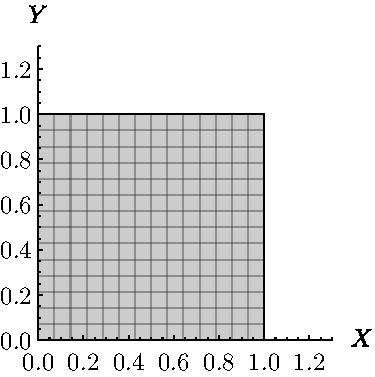
\includegraphics[width=0.4\textwidth]{images/gibanje0.pdf}
    \hspace{1em}
    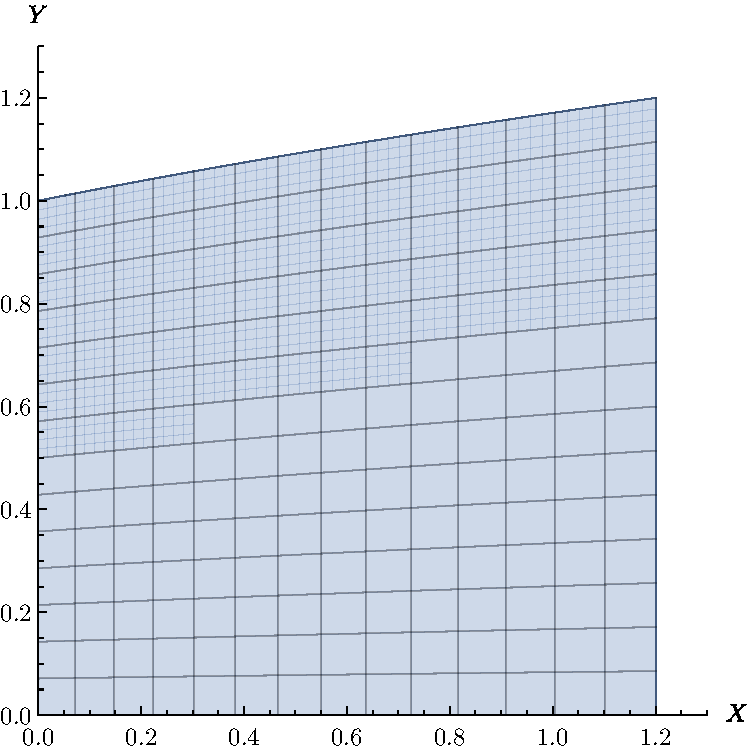
\includegraphics[width=0.4\textwidth]{images/gibanje02.pdf}
    \caption{Prerez enotske kocke pri $Z = 0$ v referenčni konfiguraciji in v prostorski
    konfiguraciji ob času $t=0.2$.}
    \label{fig:gibanje}
  \end{figure}
  Za vsak $t\geq 0$ je $\vx$ difeomorfizem, saj velja
  \[ \det\left( \dpar{\vx}{(X, Y, Z)} \right) = (1+tX)(1+2tX) > 0. \]
  Zato lahko izrazimo obratno preslikavo
  \begin{equation}
    \vX(t, x, y, z) = \left(\frac{\sqrt{4 t x+1}-1}{2 t},\frac{y
    \left(\sqrt{4 t x+1}-1\right)}{2 t x}, z\right).
    \label{eq:gibanje-inv}
  \end{equation}
\end{primer}

Vsako količino $\phi$ definirano na telesu $\B$, kot na primer temperaturo ali
hitrost, lahko zapišemo na dva načina, v
prostorskih ali v referenčnih koordinatah. Za funkcijo
\begin{align}
  \tilde \phi\colon B &\to \phi(\B) \nonumber \\
  \vX&\mapsto \phi(\chi_R^{-1}(\vX)), \label{eq:toref}
\end{align}
pravimo, da je zapisana v referenčnih koordinatah in pišemo $\tilde\phi =
\phi(\vX)$.
Podobno za funkcijo
\begin{align}
  \hat \phi\colon B_t &\to \phi(\B) \nonumber \\
  \vx&\mapsto \phi(\chi_t^{-1}(\vx)), \label{eq:topro}
\end{align}
pravimo, da je zapisana v prostorskih koordinatah in pišemo $\hat\phi = \phi(\vx)$.
Med obema zapisoma lahko prehajamo s pomočjo izražave $\phi(\vx) = \phi(\vx(t, \vX))$
ali $\phi(\vX) = \phi(\vX(\vx, t))$.

Podoben zapis bomo uporabljali tudi pri diferencialnih operatorjih. Pri odvodih
moramo povedati, ali na količino gledamo v prostorskih ali v referenčnih
koordinatah. Z velikimi črkami bomo pisali operatorje, kjer odvajamo glede na
referenčne koordinate, z malimi pa tiste, kjer odvajamo glede na prostorske.

\begin{primer}
  Damo imamo dano količino $\vartheta(t, X, Y, Z) = tX^2 + 2 ZY$, ki je zapisana v
  referenčnih koordinatah. Če jo zapišemo v prostorskih s pomočjo izpeljane
  inverzne relacije~\eqref{eq:gibanje-inv} iz primera~\ref{prim:gib} dobimo
  \[
    \vartheta(t, x, y, z) = \frac{2 t x^2+2 y z \left(\sqrt{4 t x+1}-1\right)-x
    \sqrt{4 t x+1}+x}{2 t x}.
  \]
  Da demonstriramo še uporabo diferencialnih operatorjev, izračunajmo
  \begin{align*}
    \dpar{\vartheta}{Y} &= 2Z  \\
    \dpar{\vartheta}{y} &= \frac{z \left(\sqrt{4 t x+1}-1\right)}{t x}.
  \end{align*}
  Te odvode bi zopet lahko zapisali kot funkcije referenčnih ali prostorskih
  koordinat. Podobno se obnašajo časovni odvodi.
  \begin{align*}
    \DDt{} \vartheta &= X^2 \\
    \ddt{} \vartheta &=  -\frac{\left(-2 t x+\sqrt{4 t x+1}-1\right) (x-2 y
    z)}{2 t^2 x \sqrt{4 t x+1}}.
  \end{align*}
  Če vidimo izraz $\DDt \vartheta(t, x, y, z)$, torej časovni odvod pri
  konstantnih referenčnih koordinatah  izraza izraženega v prostorskih
  koordinatah, ga izračunamo tako, da izraz prevedemo v referenčne koordinate,
  odvajamo po času in prenesemo nazaj na prostorske koordinate. S simboli
  lahko to zapišemo kot
  \[
    \left(\DDt{} \vartheta\right)(t, \vx) = \left( \DDt{}\vartheta(\vx(t, \vX))
    \right)(\vX(t, \vx)).
  \]
\end{primer}

Gibanje, kot opisano sedaj, res modelira makroskopsko gibanje kot ga poznamo iz
resničnega sveta. Pogoji gladkosti zagotavljajo, da se telesa ne morejo kar
izginiti in se pojaviti drugje, ter da se ne morejo sploščiti ali sekati samih
sebe. Sedaj definirajmo še pojma pomika, hitrosti in pospeška.

\begin{definicija}
  Količino \[ \vu(\vX) = \vx(t, \vX) - \vX \] imenujemo \emph{pomik}.
  Količino \[ \vv(\vX) = \DDt{\vx}(t, \vX) \] imenujemo \emph{hitrost}.
  Količino \[ \va(\vX) = \DDt{\vv}(t, \vX) \] imenujemo \emph{pospešek}.
\end{definicija}
\begin{trditev}
  Odvod po času v referenčnem koordinatnem sistemu se lahko direktno izračuna v
  prostorskem kot
  \[
  \DDt{\phi}(t, \vx) = \ddt{\phi}(t, \vx) + ((\grad \phi)(t, \vx)) \vv(t, \vx).
  \]
\end{trditev}
\proof
  Po definiciji najprej prenesemo $\phi$ v referenčni koordinatni sistem z
  uporabo~\ref{eq:toref}. Nato odvajamo po verižnem pravilu
  \begin{align*}
    \DDt \phi(t, \vx) &= \DDt \phi(t, \vx(t, \vX)) =
    \ddt \phi(t, \vx) + \dpar{\phi}{\vx} \DDt{\vx} (t, \vX) = \\
    &= \ddt \phi(t, \vx) + ((\grad \phi)(t, \vx)) \vv(t, \vX(\vx, t)).
  \end{align*}
\endproof

Poleg že naštetih količin pa imajo telesa tudi druge fizikalne lastnosti, kot so
masa in volumen, ki vplivajo na gibanje. Za modeliranje teh so pomagamo z
merami.

\begin{definicija}
  Predpostavimo, da imamo na $\B$ definirani dve Radonovi meri, $m$ in
  $V$, ki nam predstavljata maso in volumen. Predpostavimo še, da je $m \ll V$,
  torej, če je volumen nekega podtelesa nič, je tudi njegova masa nič. Od tod po
  Radon-Nikodymovem izreku sledi, da obstaja merljiva funkcija $\rho =
  \dd{m}{V}$, da velja
  \[
    m(A) = \int_{A} \rho dV
  \]
  za vsako merljivo podmnožico $A \subseteq \B$.
  Funkciji $\rho\colon\B\to[0, \infty)$ pravimo \emph{gostota}.
\end{definicija}
\begin{opomba}
  Ponavadi za $V$ vzamemo kar Lebesgueevo mero na $\R^3$, mero $m$ pa podamo tako, da
  podamo gostoto telesa $\rho$. Meri $m$ in $V$ s potiskom prek konfiguracij
  razširimo na referenčni in prostorski položaj.
\end{opomba}

\subsubsection{Aksiomi gibanja}
Iz mehanike točke in iz resničnega sveta vemo, da gibanje zadošča nekim
zakonom, ki jih bomo za nadaljnje izpeljave privzeli kot aksiome.

\begin{aksiom}[Zakon o ohranitvi mase]
  \label{aks:masa}
  Za vsako telo $\B$ in vsako njegovo gibanje velja
  \begin{equation}
    \DDt{}m(B_t) = 0.
    \label{eq:masa}
  \end{equation}
  Masa se med gibanjem niti ne izgublja niti ne nastaja in je vseskozi
  konstantna.
\end{aksiom}

Druga dva aksioma bosta poleg mase imela opraviti s silami. Predpostavili bomo,
da lahko sile na telo delujejo na dva načina: kot telesne sile ali pa kot
površinske sile.

\begin{definicija}
  \emph{Volumenska gostota sile} $\vf$ je zvezna funkcija $\vf\colon B_t\to\R^3$.
  \emph{Površinska gostota sile} $\vt$ je zvezna funkcija $\vt\colon\partial B_t\to\R^3$.
\end{definicija}

\begin{aksiom}[Zakon o ohranitvi gibalne količine]
  \label{aks:gib}
  Za vsako telo $\B$ velja
  \begin{equation}
    \DDt{}\int_{B_t} \vv dm = \int_{B_t} \vf dV + \int_{\partial B_t} \vec t dS.
    \label{eq:gib}
  \end{equation}
  Sprememba gibalne količine je enaka vsoti vseh sil, ki delujejo na telo.
\end{aksiom}

\begin{aksiom}[Zakon o ohranitvi vrtilne količine]
  \label{aks:vrt}
  Za vsako telo $\B$ velja
  \begin{equation}
    \DDt{}\int_{B_t}\vx \times \vv dm = \int_{B_t} \vx \times \vf dV +
    \int_{\partial B_t} \vx\times\vt dS.
    \label{eq:vrt}
  \end{equation}
  Sprememba vrtilne količine je enaka vsoti vseh zunanjih navorov, ki delujejo
  na telo.
\end{aksiom}
\begin{opomba}
  Pri aksiomu~\ref{aks:vrt} smo predpostavili, da na kontinuum ne delujejo
  notranji, ampak da so vsi navori posledica delovanja zunanjih sil. Drugače
  povedano, predpostavili smo \emph{nepolarnost} kontinuuma.
\end{opomba}

V vseh treh aksiomih nastopa odvod po času v referenčnih koordinatah nekega
integrala, zapisanega v prostorskih koordinatah. Tu ne velja običajen izrek o
odvajanju pod integralom, zato moramo izraz pod integralom najprej prenesti v
referenčne koordinate, zamenjati odvod in integral, nato pa ga prenesti nazaj.
Naredimo to najprej za aksiom o ohranitvi mase.
\begin{trditev} Masa se ohranja $(\DDt{}m(B_t) = 0)$ natanko tedaj, ko je
  \begin{equation}
    \DDt\rho + \rho\div\vv = 0.
    \label{eq:ohr-masa}
  \end{equation}
\end{trditev}
\proof
Trditev pokaže direkten račun, kjer bomo zamenjali integralsko spremenljivko iz
$\vx$ na $\vX$ in nato nazaj. Pri uvedbi nove spremenljivke se bo v integralu
pojavila determinanta $f = \det(F)$ diferenciala prehodne preslikave $F =
\dpar{\vx}{\vX}$, prav tako pa tudi njen odvod $\DDt{J}$, zato ga izračunajmo vnaprej:
\begin{align*}
  \DDt J &= \tr\left(\operatorname{adj}(F) \DDt{F}\right) =
  \tr\left(\det(F)F^{-1} \dpar{^2\vx}{\vX\partial t}\right) =
  \det(F)\tr\left(\dpar{\vv}{\vX}F^{-1}\right) = \\ &=
  \det(F)\tr\left(\dpar{\vv}{\vX}\dpar{\vX}{\vx}\right) =
  \det(F)\tr\left(\grad \vv\right) =
  \det(F)\div \vv.
\end{align*}
Pri tem smo uporabili Jacobijevo formulo za računanje odvoda
determinante, ciklično lastnost sledi, formulo za računanje odvoda inverza in verižno pravilo.
Sedaj imamo vse pripravljeno za glavni izračun.
\begin{align*}
  0 &= \DDt{}m(B_t) =
  \DDt{} \int_{B_t} dm =
  \DDt{} \int_{B_t} \rho dV =
  \DDt{} \int_{B} \rho J dV =\\ &=
  \int_{B} \DDt{}(\rho J) dV =
  \int_{B}\left( \DDt{\rho} J + \rho \DDt{J} \right)dV = \\ &=
  \int_{B}\left( \DDt{\rho}  + \rho \div\vv\right) J dV =
  \int_{B_t}\left( \DDt{\rho}  + \rho \div\vv\right) dV.
\end{align*}
Ker je integral nič za vsako telo, mora biti nujno integrand nič, in obratno, če
je integrand nič, se masa ohranja.
\endproof

Zgornjo trditev bomo s pridom uporabili pri izračunu odvoda integrala splošne
količine.
\begin{trditev}
  \label{trd:swap-der-int}
  Naj bo $\phi$ neka količina in privzemimo aksiom o ohranitvi mase. Potem
  velja
  \begin{equation}
    \DDt{} \int_{B_t}\phi dm = \int_{B_t} \DDt{\phi} dm.
    \label{eq:swap-der-int}
  \end{equation}
\end{trditev}
\proof
Postopamo enako kot v prejšnji trditvi. Izračunamo
\begin{align*}
    \DDt{} \int_{B_t}\phi dm &=
    \DDt{} \int_{B}\phi \rho J dV =
    \int_{B} \DDt{(\phi \rho J)} dV  = \\ &=
  \int_{B} \left(\DDt{\phi} \rho J + \phi \left(\underbrace{\DDt{\rho} + \rho
  \div \vv}_{=\;0 \text{ po \eqref{eq:ohr-masa}}} \right) \right)dV  = \\ &=
  \int_{B} \DDt{\phi} \rho JdV =
  \int_{B_t} \DDt{\phi} dm. \qedhere
\end{align*}
\endproof

\subsection{Napetostni tenzor}
Predstavljajmo si, da na telo deluje neka površinska sila z gostoto $\vt$. Ta sila deluje
na zunanjo površino telesa, nato pa se prenaša skozi telo od točke do točke.
Če skozi telo potegnemo namišljeno ravnino, ki ga razdeli na dva dela.
Na tej površini en del kontinuuma deluje na drug del, toda ekvivalentno bi bilo,
če bi enega izmed teh delov odstranili in na površino preostanka delovali z
enakimi silami, kot je prej deloval drugi del.

Ta razmislek nam ponuja naslednji opis notranjih in površinskih sil telesa.
V nekem trenutku $t$ v času se postavimo v neko točko $\vx$ v telesu in skozi izbrano
točko potegnemo ravnino z normalo $\vn$. Tedaj obstaja vektor $\vt$, ki
prestavlja silo, s katero kontinuum z ene strani ravnine deluje v tej točki na
tistega na drugi strani. Poleg tega, če potegnemo katero koli drugi ploskev
skozi točko $\vx$ z enako normalo $\vn$, bo vektor $\vt$, še vedno enak, saj bo
kontinuum deloval z enako silo. Temu razmisleku se reče \emph{Cauchyeva
hipoteza}.

\begin{aksiom}[Cauchyeva hipoteza]
  V telesu obstaja vektorsko polje $\vt$ inducirano s površinskimi silami, ki
  je odvisno samo od položaja, časa in normale na površino (resnično ali
  namišljeno), kjer ga opazujemo.  S simboli lahko zapišemo
  \[
    \vt = \vt(t, \vx, \vn).
  \]
\end{aksiom}

Iz zgornjega razmisleka se zdi, da bi morala biti sila, s katero prvi del
kontinuuma deluje na drugega nasprotno enaka sili, s katero drugi deluje na
prvega. Temu se reče tudi tretji Newtonov zakon za mehaniko kontinuuma in
ga ni treba privzeti kot aksiom, ampak lahko dokažemo iz do sedaj
privzetih aksiomov. Dokaza tega in naslednjega izreka bosta povzeta po dokazih
iz~\cite[str.\ 104--107]{hjelmstad2007fundamentals}.
\begin{trditev}[Cauchyeva recipročna relacija]
  \label{trd:cauchy-reciprocal}
  \begin{equation}
    \vt(t, \vx, -\vn) = -\vt(t, \vx, \vn)
    \label{eq:cauchy-reciprocal}
  \end{equation}
\end{trditev}
\proof
Izberimo trenutek v času $t$ in točko $\vx$. Krajše pišimo $\vt_{\vn} = \vt(t, \vx,
\vn)$. Oglejmo si podtelo v obliki krožnega valja z višino $h^2$ in radijem $h$, ki ima
v središču točko $\vx$ in je $\vn$ normala na eno izmed osnovnic.
Tako podtelo zaradi odprtosti $\B$ gotovo obstaja za dovolj majhen $h$. Označimo
osnovnico z normalo $\vn$ z $B^+$, nasprotno z $B^-$ in plašč s $P$. Površina
vsake osnovnice je $\pi h^2$, površina plašča pa $2 \pi h^3$. Volumen valja je
$\pi h^4$. Primer valja je prikazan na sliki~\ref{fig:valj}.

\begin{figure}[h]
  \centering
  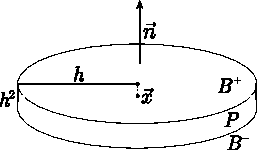
\includegraphics[width=0.4\textwidth]{images/cauchy_disc.pdf}
  \caption{Valj, uporabljen v dokazu Cauchyjeve recipročne relacije.}
  \label{fig:valj}
\end{figure}

Uporabimo za ta
valj aksiom o gibalni količini~\eqref{eq:gib}:
\begin{align*}
  \DDt{} \int_{B_t} \vv dm = \int_{B_t} \vf dV + \int_{\partial B_t} \vt dS.
\end{align*}
Zaradi gladkosti $\vv$ in ohranitve mase lahko zamenjamo odvod in integral in rob valja
razpišemo po ploskvah. Vektor $\vm(\vx)$ naj označuje normalo na plašč valja.
\[
  \int_{B_t} \DDt{\vv} \rho dV = \int_{B_t} \vf dV + \int_{B^+} \vt_{\vn} dS +
  \int_{B^-}\vt_{-\vn} dS + \int_{P} \vt_{\vm(\vx)}dS
\]
Sedaj na vsakem od integralov uporabimo izrek o povprečni vrednosti
\[
  V(B) (\rho\DDt{\vv})(\vx_1) = V(B) \vf(\vx_2) + S(B^+)\vt_{\vn}(\vx_3) +
  S(B^-)\vt_{-\vn}(\vx_4) + S(P)\vt_{\vm(\vx)}(\vx_5),
\]
kjer so $\vx_1, \vx_2, \vx_3, \vx_4, \vx_5$ neke vmesne točke v ali na površini valja.
Če vstavimo notri izraze za volumen in površine ploskev dobimo
\[
  \pi h^4 (\rho \DDt{\vv})(\vx_1) = \pi h^4 \vf(\vx_2) + \pi h^2 \vt_{\vn}(\vx_3) +
  \pi h^2 \vt_{-\vn}(\vx_4) + 2 \pi h^3 \vt_{\vm(x)}(\vx_5).
\]
Če celoten izraz delimo z $\pi h^2$ in pogledamo limito $h\to 0$ gredo vse točke
$\vx_i$ proti $\vx$ in dobimo
\[
  0 = \vt_{\vn}(\vx) + \vt_{-\vn}(\vx),
\]
kar je točno to, kar smo želeli pokazati.
\endproof

Izkaže se, da velja še več: vektor $\vt$ je linearno odvisen od normale. S
pomočjo prejšnje trditve lahko pokažemo naslednji izrek, ki nam da na voljo
matematični objekt, s pomočjo katerega lahko opišemo napetost v materialu.
\begin{izrek}[Cauchyev izrek o napetosti]
  Obstaja tenzor $\ts$, tako da velja \[
    \vt(t, \vx, \vn) = \ts(t, \vx)\vn.
  \]
  Tenzor $\ts$ se imenuje Cauchyev napetostni tenzor,
\end{izrek}
\proof
Podobno kot pri Cacuchyevi recipročni relaciji si izberimo majhno telo okoli
točke $\vx$. Tokrat naj bo to tetraeder z tremi stranicami vzporednimi
koordinatnim osem in normalo $\vn$ na ploskev, ki jo razpenjajo preostale tri
stranice, kot prikazano na sliki~\ref{fig:tetra}.

\begin{figure}[h]
  \centering
  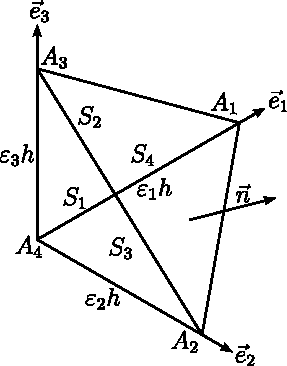
\includegraphics[width=0.4\textwidth]{images/cauchy_tetrahedron.pdf}
  \caption{Tetraeder, uporabljen za dokaz Cauchyevega izreka o napetosti.}
  \label{fig:tetra}
\end{figure}

Označimo oglišča tetraedra z $A_1, A_2, A_3, A_4 = \vx$ in ploskev nasproti izbranega
oglišča z malimi črkami $S_1, S_2, S_3, S_4$. Ploščine teh ploskev označimo z
$a_1, a_2, a_3, a_4$.  Naj bodo pravokotne stranice tetraedra
dolge $\eps_1 h$, $\eps_2 h$ in $\eps_3 h$, kjer razmerje $\eps_1 : \eps_2 : \eps_3$
določimo tako, da je normala na $S_4$ enaka $\vn$.
Celotna situacija je prikazana na sliki~\ref{fig:tetra}.
Sedaj lahko izračunamo ploščine ploskev $a_1 = \frac12 \eps_2\eps_3h^2$,
$a_2 = \frac12 \eps_1\eps_3h^2$ in $a_3 = \frac12 \eps_1\eps_2h^2$.
Volumen tetraedra je $V = \frac16 \eps_1\eps_2\eps_3h^3$.
Vektorje v smeri koordinatnih osi standardno označimo z $\ei$, $\ej$, $\ek$.
Zunanja normala na ploskev $S_1$ je $-\ei$, na ploskev $S_2$ je $-\ej$ in na
ploskev $S_3$ je $-\ek$. Normalo na preostalo ploskev, ki bo dolga ravno toliko,
kot je ploščina te ploskve, dobimo s pomočjo vektorskega produkta
stranic, ki jo oklepata.
\begin{align*}
  a_4\vn &= \frac12 (\eps_1h \ei - \eps_2h \ej) \times (\eps_3h \ek - \eps_2h
  \ej) = \\ &=
  -\frac12 \eps_2\eps_3 h^2\ei
  -\frac12 \eps_1\eps_3 h^2\ej
  -\frac12 \eps_1\eps_2 h^2\ek = \\
  &= a_1 \ei + a_2 \ej + a_3 \ek.
\end{align*}
Če to pomnožimo z $i$-tim baznim vektorjem, dobimo $a_i = (\vn\cdot\vec{e}_i)
a_4$.
Zopet uporabimo aksiom~\ref{aks:gib} o ohranitvi gibalne količine in izrek o
povprečni vrednosti
\begin{align*}
  \DDt{} \int_{B_t} \vv dm &= \int_{B_t} \vf dV + \int_{\partial {B_t}} \vt dS \\
\int_{B_t} \rho\DDt{\vv} dV &= \int_{B_t} \vf dV +
  \int_{S_1} \vt_{-\ei} dS +
  \int_{S_2} \vt_{-\ej} dS +
  \int_{S_3} \vt_{-\ek} dS +
  \int_{S_4} \vt_{\vn} dS
  \\
  V (\rho\DDt{\vv})(\vx_1) &= V \vf(\vx_2) +
  a_1 \vt_{-\ei}(\vx_3) + a_2 \vt_{-\ej}(\vx_4) + a_3 \vt_{-\ek}(\vx_5) + a_4
  \vt_{\vn}(\vx_6),
\end{align*}
pri čemer so $\vx_i$ kot v prejšnjem dokazu neke točke v notranjosti ali na
površini tetraedra. Sedaj enačbo delimo s $a_4$ in pošljemo limito $h \to 0$.
Vse točke $\vx_i$ limitirajo proti $\vx$, člena, ki vsebujeta volumen tetraedra,
pa se približujeta 0. Z upoštevanjem
\[
  \lim_{h\to0} \frac{a_i}{a_4} = \lim_{h\to0}\frac{(\vn\cdot\vec{e}_i) a_4}{a_4}
  = \vn\cdot\vec{e}_i
\]
dobimo
\[
  0 = \vt_{\vn} + \sum_{i=1}^3 (\vn \cdot\vec{e}_i) \vt_{-\vec{e}_i}.
\]
Uporabimo še Cauchyevo recipročno relacijo~\eqref{eq:cauchy-reciprocal} in dobimo
\[
  \vt_{\vn} = \sum_{i=1}^3 (\vn \cdot\vec{e}_i) \vt_{\vec{e}_i}.
\]
Ta zveza nam pove, kako je napetost na poljubni ploskvi povezana z napetostmi na
koordinatnih ploskvah.
To nam dovoljuje definicijo \emph{Cauchyevega napetostnega tenzorja}
$\ts$
\[
  \ts = \sum_{i=1}^3 \vt_{\vec{e}_i}\otimes \vec{e}_i.
\]
za katerega res velja
\[
  \ts\vn = \sum_{i=1}^3 (\vt_{\vec{e}_i}\otimes \vec{e}_i)(\vn) =
  \sum_{i=1}^3 (\vn \cdot\vec{e}_i) \vt_{\vec{e}_i} = \vt_{\vn}. \qedhere
\]
\endproof

\subsection{Enačbe gibanja}
V tem razdelku bomo iz aksiomov izpeljali lokalne enačbe gibanja, tako da jih
bomo iz integralske oblike prevedli v diferencialno.
Prevedimo najprej aksiom~\ref{aks:gib} o ohranitvi gibalne količine.
\begin{izrek}[Cauchyeva momentna enačba]
  Za gibanje kontinuuma velja Cauchyeva momentna enačba
  \begin{equation}
    \rho \DDt{\vv} = \vf + \div \sigma.
    \label{eq:cauchy-moment}
  \end{equation}
\end{izrek}
\proof
Za vsako telo s prostorsko konfiguracijo $B_t$ velja
\begin{align*}
  \DDt{} \int_{B_t} \vv dm &= \int_{B_t} \vf dV + \int_{\partial {B_t}} \vt dS \\
  \int_{B_t} \DDt{\vv}\rho dV &= \int_{B_t} \vf dV + \int_{\partial {B_t}} \ts \vn dS \\
  \int_{B_t} \DDt{\vv}\rho dV &= \int_{B_t} \vf dV + \int_{B_t} \div \ts dV \\
  0 &= \int_{B_t}\left(\DDt{\vv}\rho - \vf - \div \ts\right) dV. \\
\end{align*}
V računu smo uporabili Gaussov izrek~\ref{izr:gauss} za tenzorje drugega reda in
izrek~\ref{trd:swap-der-int} o menjavi odvoda in integrala. Ker mora biti končni
integral nič za vsako telo, mora biti integrand nič, kar dokaže našo enačbo.
\endproof

Do sedaj še nismo uporabili aksioma~\ref{aks:vrt} o vrtilni količini.
Njegova lokalna oblika se prevede na zelo enostavno trditev o simetriji
Cauchyevega napetostnega tenzorja.
\begin{trditev}
  \label{trd:sigma-symmetric}
  Cauchyev napetostni tenzor je simetričen:
  \[ \ts^\T = \ts. \]
\end{trditev}
\proof
Začnimo z zakonom o vrtilni količini~\eqref{eq:vrt} in ga prevedimo v lokalno
obliko.
\begin{align*}
  \DDt{}\int_{B_t}\vx \times \vv dm = \int_{B_t} \vx \times \vf dV +
  \int_{\partial B_t} \vx\times\vt dS.
\end{align*}
Posvetimo se zadnjemu členu in ga pomnožimo s konstantnih vektorjem $\vw$:
\begin{align*}
\left(\int_{\partial B_t} \vx \times \vt dS\right)\cdot \vw  &=
  \int_{\partial B_t} \langle \vx, \vt, \vw \rangle dS =
  \int_{\partial B_t} \langle \vw, \vx, \vt \rangle dS = \\ &=
  \int_{\partial B_t} (\vw \times \vx) \cdot \vt dS =
  \int_{\partial B_t} (\vw \times \vx) \cdot \ts\vn dS = \\ &=
  \int_{\partial B_t} \ts^\T(\vw \times \vx) \cdot d\vec{S} =
  \int_{\partial B_t} \ts^\T(\vw \times \vx) \cdot d\vec{S} = \\ &=
  \int_{B_t} \div (\ts^\T(\vw \times \vx)) dV = \\ &=
\int_{B_t} [\langle \div \ts, \vw, \vx\rangle +  \ts : \grad (\vw \times \vx)] dV.
\end{align*}
Zgoraj smo uporabili po vrsti: definicijo in cikličnost mešanega produkta, definicijo
$\ts^\T$, Gaussov izrek in relacijo iz trditve~\ref{trd:div-tv}.

Podobno z $\vw$ pomnožimo tudi zakon o vrtilni količini in vstavimo zgornjo
relacijo.
\begin{align*}
  0 &= \left(\DDt{}\int_{B_t}\vx \times \vv dm - \int_{B_t} \vx \times \vf dV -
  \int_{\partial B_t} \vx\times\vt dS\right)\cdot \vw = \\ &=
  \DDt{}\int_{B_t}\langle \vx, \vv, \vw\rangle  dm - \int_{B_t} \langle \vx,
  \vf, \vw\rangle dV - \int_{B_t} [\langle \div \ts, \vw, \vx\rangle +  \ts :
  \grad (\vw \times \vx)] dV = \\ &=
  \int_{B_t}\langle \rho \DDt\vv, \vw, \vx \rangle  dV - \int_{B_t} \langle \vf,
  \vw, \vx\rangle dV - \int_{B_t} [\langle \div \ts, \vw, \vx\rangle +  \ts :
  \grad (\vw \times \vx)] dV = \\ &=
\int_{B_t}\left[ \left\langle\rho \DDt\vv - \vf - \div \ts, \vw, \vx\right\rangle -  \ts : \grad
  (\vw \times \vx)\right] dV = \\ &=
- \int_{B_t} \ts : \grad (\vw \times \vx) dV.
\end{align*}
Uporabili smo definicijo in cikličnost mešanega produkta, Cauchyevo momentno
enačbo~\eqref{eq:cauchy-moment} in dejstvo, da je
\[
  \DDt{}\langle \vx, \vv, \vw \rangle =
  \langle \vv, \vv, \vw \rangle +
  \langle \vx, \DDt\vv, \vw \rangle =
  \langle \DDt\vv, \vw, \vx \rangle.
\]
Ker aksiom o vrtilni količini drži za vsako telo, mora biti
\[
  \ts : \grad (\vw \times \vx) = 0,
\]
za poljuben vektor $\vw$. Tenzor $\grad (\vw \times \vx)$ je antisimetričen in
vsak antisimetričen tenzor lahko s pomočjo njegovega osnega vektorja zapišemo v
tej obliki, zato je zgornja relacija ekvivaletna trditvi, da je, zato je zgornja
relacija ekvivaletna trditvi, da je
\[ \ts : w = 0\] za vsak antisimetričen tenzor $w$.
Torej je $\ts \in Asym(\R^3)^\perp$ in po trditvi~\ref{trd:dot-antisym-tensor}
mora biti $\ts$ simetričen.
\endproof

\subsection{Konstitutivne enačbe}
Do sedaj izpeljane enačbe veljajo za poljuben kontinuum, naj bo to tekočina,
plastična ali elastična trdnina. V tem razdelku si bomo ogledali enačbe, ki
definirajo obnašanje našega kontinuuma kot elastične trdnine preko posplošitve
Hookovega zakona, ki povezuje napetosti in deformacijo. Naučili smo se že, kako
izražamo napetost, sedaj pa si poglejmo, kako merimo deformacijo teles.
Tukaj bomo tudi privzeli, da je referenčna konfiguracija kar prostorska
konfiguracija na začetku gibanja.

\subsubsection{Mera deformacije}
\begin{definicija}[Gradient deformacije]
  Količino $F = \dpar{\vx}{\vX}(t, \vX) = \Grad \vx$ imenujemo \emph{gradient
  deformacije}.
\end{definicija}

Tenzor $F$ je drugega reda in nam v vsaki točki predstavlja lokalno deformacijo
telesa. Privzeli smo že, da je $\vx$ difeomorfizem, torej je $F$ neizrojev,
dodatno pa bomo privzeli še, da gibanje $\vx$ \emph{ohranja orientacijo}, saj
so gibanja realnih teles taka. Od tod sledi, da je $\det F > 0$.
Fizikalno interpretacijo $F$ dobimo z naslednjim Taylorjevim ravojem:
\[
  d\vx := \vx(t, \vX+d\vX) - \vx(t, \vX) = F d\vX + O(d\vX^2).
\]
Tenzor $F$ do prvega reda natančno opiše kako se vektor $d\vX$ iz referenčne
konfiguracije deformira v vektor $d\vx$ v prostorski konfiguraciji.

Vendar, ni vsa deformacija, ki jo opiše tenzor $F$ taka, da bi povzročala
napetosti. Hookov zakon v eni dimenziji pravi, da je sila sorazmerna raztezku.
Če imamo opravka s togim premikom $\vX \mapsto Q\vX + a$, ta premik ne bo povzročil
nobene napetosti, saj se bo telo samo premaknilo, ne pa raztegnilo.

Oglejmo si najprej primer v eni dimenziji.
\begin{primer}
Naj bo dana tanka palica kot na sliki~\ref{fig:palica}, ki jo raztegnemo vzdolž
njene nosilke.
\begin{figure}[h]
  \centering
  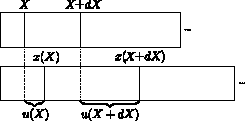
\includegraphics[width=0.55\textwidth]{images/stretch1d.pdf}
  \caption{Razteg tanke palice vzdolž njene osi.}
  \label{fig:palica}
\end{figure}
Premik v točki $\vX$ je $u(\vX) = \vx - \vX$, v točki $\vX+d\vX$ pa $u(\vX+d\vX)$.
Dejanski relativni raztezek delčka palice dolžine $d\vX$ pa je
\begin{align*}
  \frac{d\vx - d\vX}{d\vX} &= \frac{\vx(\vX+d\vX) - \vx(\vX) - (\vX + d\vX - \vX)}{d\vX} = \\ &=
  \frac{\vu(\vX + d\vX) - \vu(\vX)}{d\vX} = \vu'(\vX) + O(d\vX).
\end{align*}
Do prvega reda je relativni raztezek v točki $\vX$ enak kar $u'(\vX)$.

Preverimo še, da ta mera raztezka zadošča nekaterih intuitivnim zahtevam. Za
togi premik $\vX \mapsto \vX + c$ je $\vu(\vX) = c$ in $\vu'(\vX) \equiv 0$, kot
pričakovano.

Za enakomerni razteg $\vX \mapsto a\vX$ je $\vu(\vX) = a\vX - \vX$ in $\vu'(\vX) = a - 1$. Tudi
to ustreza pričakovanjem, saj za $a = 1$ ni raztezka, za $a< 1$ je to skrčitev
in je raztezek negativen, za $a>1$ pa dobimo pozitivno število.
\end{primer}

Analogna mera deformacije med točkama $\vX$ in $\vX+d\vX$ v višji dimenziji bi bila
\[
  \eps_1 = \frac{\|d\vx\| - \|d\vX\|}{\|d\vX\|}.
\]
Toda veliko lažje je računati s kvadrati norm kot z normami vektorjev, zato je
bolj primerna mera
\[
  \eps_2 = \frac{\|d\vx\|^2 - \|d\vX\|^2}{\|d\vX\|^2}.
\]
Ker velja $\eps_2 = (1+\eps_1)^2 - 1 = 2\eps_1 + \eps_1^2$ je za majhne pomike
$\eps_2 \approx 2\eps_1$ in sta meri ekivalentni.

Izračunajmo infinitezimalno aproksimacijo mere $\eps_2$.
\begin{align*}
  \eps_2 &=
  \frac{\|d\vx\|^2 - \|d\vX\|^2}{\|d\vX\|^2} =
  \frac{\|d\vx\|^2}{\|d\vX\|^2}  - 1=
  \frac{\|F d\vX + O(d\vX^2)\|^2}{\|d\vX\|^2} - 1 = \\ &=
  \frac{d\vX^\T F^\T F d\vX + O(d\vX^3)}{\|d\vX\|^2} - 1 =
  \frac{d\vX}{\|d\vX\|}(\underbrace{F^\T F - I}_{2E})\frac{d\vX}{\|d\vX\|} + O(d\vX)
\end{align*}
V limiti $d\vX \to 0$ lahko mero $\eps_2$ predstavimo s tenzorjem $F^\T F- I$,
mero $\eps_1$ pa s tenzorjem $E$.

\begin{definicija}[deformacijski tenzor]
  Količina $E = \frac12 (F^\T F - I)$ se imenuje (Cauchy-Greenov)
  deformacijski tenzor.
\end{definicija}
\begin{trditev}
  Deformacijski tenzor $E$ lahko izrazimo z gradientom pomika kot
  \[ E = \frac12\left( \Grad \vu + \Grad \vu^\T + \Grad \vu^\T \Grad \vu \right). \]
\end{trditev}
\proof
Trditev pokaže preprost račun. Spomnimo se, da je pomik definiran kot $\vu(\vX) =
\vx(\vX) - \vX$ in je gradient pomika enak
\[
  \Grad \vu(\vX) = \dpar{\vu}{\vX} = \dpar{\vx}{\vX} - I = F - I.
\]
Izračunamo:
\begin{align*}
  &\frac12\left( \Grad \vu + \Grad \vu^\T + \Grad \vu^\T \Grad \vu \right) = \\
  &\qquad=\frac12\left(F - I + F^\T - I  + (F-I)^\T(F-I)\right) = \\
  &\qquad=\frac12\left(F + F^T - 2I + F^\T F - F - F^T + I\right) = \\
  &\qquad=\frac12\left(F^\T F - I\right) = \\
  &\qquad=E.\qedhere
\end{align*}
\endproof

Deformacijo $F$ lahko z pomočjo polarnega razcepa zapišemo kot $F = RU$, kjer je
$R$ ortogonalna in $U$ pozitivno definitna matrika. Tenzor $R$ predstavlja
rotacijo, $U$ pa razteg in strig. Predstavljamo si lahko, da je deformacijo $F$
izvedemo tako, da najprej telo raztegnemo in strižno deformiramo, nato pa
zavrtimo v končno lego.

Rotacija $R$ ne vpliva na rabo materiala, saj je deformacija toga in ne povzroča
notranjih napetosti. Prava mera deformacije, ki vpliva na napetost v materialu
torej ne vsebuje nobenih rotacij. Za mero deformacije bi lahko vzeli kar to,
koliko se $U$ razlikuje od identitete, toda polarni razcep matrike je težko
izračunati. Poglejmo si kakšno zvezo ima zgoraj definirani deformacijski tenzor
$E$ z $U$:
\[
  E = \frac12(f^\T F - I) = \frac12(U^\T R^\T R U - I) = \frac12 (U^2 - I).
\]
Vidimo, da $E$ meri, kako se $U^2$ razlikuje od identitete, ki predstavlja
gibanje brez deformacij.

Kot pri enodimenzionalnem primeru si oglejmo, kako se $E$ obnaša pri enostavnih
deformacijah. Za toge premike imamo želeno obnašanje, kot pokazano v naslednji
trditvi.

\begin{primer}
  Kot prej si oglejmo, da je za toge deformacije $E = 0$.
 Naj bo deformacija toga, torej oblike $\vX \mapsto Q\vX +
c$ z ortogonalno konstantno matriko $Q$ in konstantnim $c$. Tedaj je
\[ E = \frac12 (F^\T F - I) = \frac12(Q^\T Q - I) = \frac12(I - I) = 0. \]
Oglejmo si še enostavni razteg v smeri osi, dan kot
$\vX \mapsto \diag(\lambda_1, \lambda_2, \lambda_3) \vX$.
V tem primeru velja $F = \diag(\lambda_1, \lambda_2, \lambda_3)$ in
  \[
    E = \diag\left(
      \frac{\lambda_1^2-1}{2},
      \frac{\lambda_2^2-1}{2},
      \frac{\lambda_3^2-1}{2}
    \right).
  \]
  Če je $\lambda_i = 1$ je $E$ res 0, sicer pa so v njegovih diagonalnih
  komponentah zapisani raztezki vzdolž posameznih osi.
\end{primer}

V teoriji linearne elastičnosti se bomo ukvarjali z majhnimi pomiki in majhnimi
gradienti pomikov. Zato poenostavimo deformacijski tenzor z geometrijsko
linearizacijo: zanemarimo člen $\Grad \vu^\T \Grad \vu$.

\begin{definicija}[infinitezimalni deformacijski tenzor]
  Količino
  \begin{equation}
    \eps = \frac{1}{2}(\Grad \vu + \Grad \vu^\T)
    \label{eq:eps}
  \end{equation}
  imenujemo \emph{infinitezimalni deformacijski tenzor}, ki je geometrijska
  linearizacija deformacijskega tenzorja.
\end{definicija}

% \begin{trditev}
%   Če za gibanje velja $\eps = 0$, potem je pomik oblike $u = \va + \vb \times
%   X$, za konstantna vektorja $\va$ in $\vb$.
% \end{trditev}
% \proof
% Iz $\eps = 0$ direktno sledi $\Grad u = -\Grad u^\T$. Ker je $\Grad u$
% antisimetričen, obstaja osni vektor $\vb$, tako da velja $(\Grad u) \vv = \vb
% \times \vv$ za vsak vektor $\vv$.
% \endproof

\subsubsection{Hookov zakon}
Sedaj potrebujemo relacijo, ki povezuje premike z napetostjo.
V splošnem je relacija oblike $\ts = f(\eps)$, predpostavimo torej, da je
napetost odvisna samo od deformacije. Ponavadi $f$ dodatno omejimo, da je
izotropična in da mora biti zveza taka, da je energija
\[
  U(\eps) = \int_{0}^{\eps} \ts : d\eps = \int_0^\eps f(\eps) d\eps
\]
dobro definirana, torej neodvisna od poti integracije. V tem primeru je
\[
  \ts = \dpar{U(\eps)}{\eps}.
\]
Če to drži, pravimo, da je material hiperelastičen, kot pravi naslednja
definicija.
\begin{definicija}
  Material je \emph{hiperelastičen}, če je $U(\eps) = \int_0^\eps \ts:d\eps$ neodvisen
  od poti integracije.
\end{definicija}
V teoriji linearne elastičnosti
predpostavimo, da je zveza $f$ med naptostjo in deformacijo linearna in jo
imenujemo Hookov zakon, saj je posplošitev običajnega Hookovega zakona za vzmet.
\begin{aksiom}[Hookov zakon]
  \label{aks:hook}
  Napetost je linearno odvisna od deformacije, preko tenzorja četrtega reda $C$:
  \[ \ts = C:\eps. \]
  Tenzor $C$ se imenuje \emph{tenzor elastičnosti} ali togostni tenzor
  \ang{stifness tensor} in ima v splošnem $3^4 = 81$ prostih parametrov.
\end{aksiom}
\begin{opomba}
  Aksiom~\ref{aks:hook} se po komponentah glasi $\ts_{ij} = C_{ijkl}
  \eps_{kl}$.
\end{opomba}
Na srečo v splošnem $C$ nima 81 prostih komponent.
Iz trditve~\ref{trd:sigma-symmetric} o simetričnosti $\ts$ sledi, da lahko
prosto zamenjamo indeksa $i$ in $j$ in velja $C_{ijkl} = C_{jikl}$.
Podobno iz simetričnosti $\eps$ sledi, da je $C_{ijkl} = C_{ijlk}$.
S tem smo $C$ reducirali na $6^2 = 36$ komponent.
Če dodatno predpostavimo še hiperelastičnost, vidimo, da je $\dpar{U}{\eps_{ij}}
= \sigma_{ij} = C_{ijkl}\eps_{kl}$ in
\[
  \dpar{U}{\eps_{ij}\eps_{kl}} = C_{ijkl}.
\]
Ker vrstni red drugih odvodov ni pomemben, je $C_{ijkl} = C_{klij}$.
S tem smo $C$ reducirali na $36-5-4-3-2-1 = 21$ komponent.
Od sedaj naprej bomo predpostavili, da so vsi materiali hiperelastični.
Energija je v tem primeru dana s kvadratično formo
\begin{equation}
  U = \frac12 \eps:C:\eps.
  \label{eq:energy}
\end{equation}
Tenzor $C$ se dodatno poenostavi, če predpostavimo, da je material
\emph{izotropičen}, torej ``enak v vse smeri''. Splošen izotropičen tenzor
četrtega reda je oblike
\[
  C_{ijkl} = \lambda \delta_{ij}\delta_{kl} + \mu \delta_{ik}\delta_{jl} +
  \kappa \delta_{il}\delta_{jk},
\]
dokazano npr. v ?? in razardi zgordnjih simetrij mora veljati $\kappa =
\lambda$.
Nekoordinatno lahko sedaj zvezo $\ts = C:\eps$ za tak tenzor zapišemo kot
\begin{equation}
  \ts = \lambda (\tr\eps)I + 2\mu \eps.
  \label{eq:hooke-isotropic}
\end{equation}
Paramatra $\lambda$ in $\mu$ imenujemo Lam\'{e}jevi konstanti.
Običajno so materiali tudi homogeni, torej snovne konstante niso odvisne od
lokacije v materialu, temveč so lastnosti materiala samega.
Veliko resničnih gradbenih materialov kot na primer železo, jeklo, aluminij in
ostale kovine ter steklo. Primer anizotropnega materiala je recimo les.
V strojniških priročnikih najdemo snovne lastnosti bolje pogosto opisane s
parametroma $E$ in $\nu$, ki jima pravimo Youngov (prožnostni) modul in
Poissonovo razmerje. Zveza med njimi je
\[
  E = \frac{\mu(3\lambda+2\mu)}{\lambda+\mu} \qquad \nu =
  \frac{\lambda}{2(\lambda+\mu)}.
\]
Pogosto najdemo tudi druge snovne paramtere kot na primer strižni modul ali
stisljivost. Tabela pretvorb med različnimi parametri je na voljo v~\cite[tabela
5.1, str.\ 215]{slaughter2012linearized}. Omejitev za parametre je dana s tem,
da zahtevamo pozitivno definitnost energije kot kvadratne forme in velja natanko
tedaj, ko je $\lambda, \mu > 0$ ali pa $E > 0$ in $-1 < \nu < \frac12$.
V praksi se izkaže, da temu brez težav zadostimo. Vrednosti parametrov za nekaj
pogostih materialov so podane v tabeli~\ref{tab:Enu} in jih lahko najdemo v
primernem fizikalen ali strojnišekm priročniku, npr.~??.
\begin{table}[h]
  \centering
  \begin{tabular}{|l|l|l|} \hline
    material & $E$ [\unit{GPa}] & $\nu$ \\ \hline
    jeklo    & 210 & 0.30 \\
    aluminij & 69 & 0.33 \\
    steklo   & 50 -- 90 & 0.20 -- 0.27 \\ \hline
  \end{tabular}
  \caption{Vrednosti elastičnih parametrov za pogoste materiale.}
  \label{tab:Enu}
\end{table}

\subsection{Navierova enačba}
Sedaj imamo vse pripravljeno za opis teorije linearne elastičnosti:
\begin{enumerate}[\indent 1)]
  \item mera deformacije: $\eps = \frac12(\Grad \vu + \Grad \vu^\T)$,
  \item konstitutivna zveza: $\ts = C : \eps$ in
  \item gibalna enačba: $\rho \DDt{\vv} = \vf + \div \ts$.
\end{enumerate}

Naredimo še nekaj poenostavitev. Ker so gradienti pomikov majhni,
za poljubno količino $\phi$ velja
\begin{align*}
  \Grad\phi &= \dpar{\phi}{\vX} = \dpar{\phi}{\vx} \dpar{\vx}{\vX} = \grad\phi
  (I + \Grad u) \approx \grad \phi.
\end{align*}
Zaradi majhnih gradientov pomika je vseeno ali uporabljamo odvode glede na
prostorske ali glede na referenčne koordinate. Enak argument lahko uporabimo
tudi za divergenco in običajne odvode.

Cauchyevo gibalno enačbo lahko zapišemo namesto v prostorskih tudi v referenčnih
koordinatah. Pri tem lahko zaradi majhnih gradientov pomikov namesto $\div$
pišemo $\Div$ in Cauchyev napetostni tenzor enačimo z napetostnim tenzorjem
zapisanim v referenčnem sistemu. Opustimo tudi strogo ločevanje referenčnih in
prostorskih koordinat, saj bomo imeli od sedaj naprej enačbe vedno zapisane v
referenčnih in odvode po času pišemo s piko, za operatorje pa uporabljamo
običajne male črke ali pa kar $\nabla$.

S temi poenostavitvami dobimo \emph{linearizirano enačbo gibanja}, ki pravi
\begin{equation}
  \rho \ddot{\vu}(t, \vX) = \vf(t, \vX) + \div\sigma(t, \vX).
  \label{eq:gib-lin}
\end{equation}

Sedaj imamo vse pripravljeno, da napišemo končno enačbo, ki ji ustreza pomik
materiala. Z njeno pomočjo lahko glede na dane sile na površini in pomike na
robu izračunamo pomike v celotnem telesu, preko deformacijskega tenzorja in
Hookovega zakona pa tudi napetosti.
\begin{izrek}[Navierova enačba]
  Če so gradienti pomikov v linearno elastičnem hiperelastičnem
  izotropičnem homogenem nepolarnem mediju majhni, potem za njih velja
  \emph{Navierova enačba}
  \begin{equation}
    \rho \ddot{\vu} = \vf + (\lambda + \mu)\grad\div \vu + \mu \lap \vu.
    \label{eq:navier}
  \end{equation}
\end{izrek}
\proof
Od linearne enačbe gibanja~\eqref{eq:gib-lin} do Navierove enačbe nas loči le še
izračun $\div \sigma$. Za primerjavo naredimo izračun koordinatno in
nekoordinatno.
\begin{align*}
  \eps_{ij} &= \frac12 (\grad u)_{ij} + \frac12 (\grad u^\T)_{ij} =
  \frac12 u_{i,j} + \frac12 u_{j,i} \\
  \ts_{ij} &= \lambda \eps_{kk} \delta_{ij} + 2 \mu \eps_{ij} =
  \lambda \frac{1}{2} (u_{k,k} + u_{k,k}) \delta_{ij} + 2 \mu( \frac12 u_{i,j} +
  \frac12 u_{j,i}) =  \\ &= \lambda u_{k, k}\delta_{ij} + \mu (u_{i,j} +u_{j,i})
  \\
  (\div \ts)_i &= \sigma_{ij,j} = \lambda u_{k, kj}\delta_{ij} + \mu (u_{i,jj}
+u_{j,ij}) = \lambda u_{k,ki} + \mu (u_{i,kk} + u_{k,ki}) = \\
&= (\lambda + \mu)u_{k,ki} + \mu u_{i,kk} = (\lambda+\mu)(\grad(u_{k,k}))_i +
\mu (\lap u)_i = \\ &=
((\lambda + \mu)\grad\div u + \mu \lap u)_i
\end{align*}

Nekoordinatni dokaz pa potrebuje nekaj dodatnih relacij iz
razdelka~\ref{sec:uvod-tenz} glede diferencialnih operatorjev, ki jih bomo
uporabili v spodnjem izračunu.
\begin{align*}
  \div\ts &= \lambda \div \tr(\eps) I + 2\mu \div \eps = \\ &=
  \lambda \frac12(\div((\tr\grad u)I) + \div\tr\grad u^\T) + \mu \div(\grad u + \grad
  u^\T) = \\
  &= \frac{\lambda}{2} (\div((\div u) I) + \div( (\div u)I)) + \mu \lap u + \mu
  \grad \div u = \\
  &= \lambda \grad \div u + \mu \grad \div u + \lap u
\end{align*}
Izračun prinese enak rezultat kot prej in izrek je še enkrat dokazan.
\endproof

\subsection{Obstoj in enoličnost rešitve}
Izrek povzet po~\cite[izrek 3.15.1, str.\ 226]{lebedev2009introduction}
Prevedemo na Riezsov izrek.

\subsection{Priprava na numerično reševanje}
Za numerično reševanje se postavimo v kartezični koordinatni sistem.
Komponente tenzorja $\ts$ razpišimo:
\[
  \ts =
  \begin{bmatrix}
    \ts_{xx} & \ts_{xy} & \ts_{xz} \\
    \ts_{xy} & \ts_{yy} & \ts_{yz} \\
    \ts_{xz} & \ts_{yz} & \ts_{zz} \\
  \end{bmatrix},
\]
pri čemer smo že upoštevali simetrijo. Reševati tridimenzionalne enačbe je težje
kot dvodimenzionalne, zato si oglejmo dve poenostavitvi.

\subsubsection{Poenostavitev na dve dimenziji}
Tridimenzionalne probleme se zavoljo lažje formulacije, manjše računske
zahtevnosti in lažje implementacije pogosto s pomočjo neke simetrije prevede na
nižjedimnenzionalne. Spodaj sta opisani dve najbolj pogosti poenostavitvi.

\begin{description}
  \item[Ravninska napetost:]
Pri tej poenostavitvi predpostavimo, da napetost nima neničelnih komponent v
smeri ene izmed koordinatnih osi, torej, po primerni rotaciji koordinatnega
sistema, da so komponente $\ts_{xz}, \ts_{yz}$ in $\ts_{zz}$ enake 0. Ta
poenostavitev je primerna za telesa, ki so ``tanke plošče'', torej, imajo eno
dimenzijo veliko manjšo od ostalih dveh. Poleg tega morajo biti vse obremenitve
vzdolž plošče.
  \item[Ravninska deformacija:]
Pri tej poenostavitvi predpostavimo, da deformacijski tenzor $\eps$ nima
komponent v eni izmed koordinatnih smeri, torej, podobno kot pri ravninski
napetosti lahko predpostavimo, da so $\eps_{xz}, \eps_{yz}$ in $\eps_{zz}$ enaki
0. Ta poenostavitev je primerna za telesa, ki imajo eno dimenzijo mnogo večjo od
drugih iz se vzdolž nje ne spreminjajo, torej za (ne nujno krožne) valje.
\end{description}

Pri obeh poenostavitvah se iz pogojev izpelje, da v Navierovi enačbi ne nastopa
tretja komponenta $u$. Še več poenostavitvi sta celo ekvivalentni, saj se
razlikujeta le za konstantni člen pred enem izmed faktorjev. V dveh dimenzijah
pišemo prvo komponento pomika z $u$ in drugo z $v$, koordinati pa označujemo z
$x$ in $y$. Če si razpišemo izraze za deformacijski tenzor in napetostni tenzor
za primer ravninske napetosti dobimo:
\begin{align*}
  \eps &=
  \begin{bmatrix}
    \dpar{u}{x} & \frac12(\dpar{u}{y} + \dpar{v}{x}) \\
    \frac12(\dpar{u}{y} + \dpar{v}{x}) & \dpar{v}{y} \\
  \end{bmatrix}
  \\
  \ts &=
  \begin{bmatrix}
    \lambda \dpar{v}{y} + (\lambda+2\mu) \dpar{u}{x} &
    \mu(\dpar{u}{y} + \dpar{v}{x}) \\
    \mu(\dpar{u}{y} + \dpar{v}{x}) &
    \lambda \dpar{u}{x} + (\lambda+2\mu) \dpar{v}{y}
  \end{bmatrix}.
  \\
\end{align*}

\subsubsection{Robni pogoji}
Pri reševanju robnih problemov bomo imeli tri vrste robnih pogojev. Dirichletove
robne pogoje $u|_{\partial \Omega} = u_0$ bomo uporabili, ko bomo poznali
pomike na robu. Najpogosteje bo pogoj oblike $u = 0$, ko nek konec držimo
fiksen. Pri drugi vrsti robnih pogojev poznamo napetosti na robovih.
Najpogosteje bomo podali kar napetost na robu $\vt = \vt_0$, kjer je $\vt_0$
neka znana vrednost, npr. 0, če je ta rob prost. Tretja vrsta pogojev bodo
simetrijski pogoji, ko bomo problem reducirali preko neke osi simetrije, na osi
pa bomo zahtevali kompatibilnostne pogoje.

Oglejmo si bolj natančno pogoje, podane z napetostjo. Napetost na robu
izračunamo preko napetostnega tenzorja, $\vt = \ts\vn$, kjer ne $\vn$ zunanja
normala na rob. Za primer desnega roba, na katerega enakomerno deluje neka gostota
sile $p$ v normalni smeri dobimo dva pogoja:
\[
   \vt = \ts\vn =
  \begin{bmatrix}
    \lambda \dpar{v}{y} + (\lambda+2\mu) \dpar{u}{x} &
    \mu(\dpar{u}{y} + \dpar{v}{x}) \\
    \mu(\dpar{u}{y} + \dpar{v}{x}) &
    \lambda \dpar{u}{x} + (\lambda+2\mu) \dpar{v}{y}
  \end{bmatrix}
  \begin{bmatrix}
    1 \\ 0
  \end{bmatrix}
  =
  \begin{bmatrix}
    p \\ 0
  \end{bmatrix}.
\]

\section{Numerična metoda}
\label{sec:numericna-metoda}

V 20.~stoletju je skupaj z razvojem računalnikov začel svojo pot razvoj numeričnih
metod za reševaje parcialnih diferencialnih enačb. Do danes je bilo razvitih
veliko metod za numerično reševanje parcialnih diferencialnih enačb. Dva
pomembna razreda metod se ločita glede na obliko v kateri rešujemo parcialno
diferencialno enačbo: šibki~\ang{weak form} ali močni~\ang{strong form}.
Najznamenitejši in zelo uspešen predstavnik prve skupine je metoda končnih
elementov (MKE)~\ang{finite element method (FEM}, kjer problem najprej prevedemo
v šibko obliko, nato pa rešitev poiščemo kot linearno kombinacijo baznih
funkcij iz izbranega prostora. Najbolj poznan, predstavnik druge pa je metoda
končnih diferenc (MKD)~\ang{finite diference method (FDM)}, pri kateri
direktno diskretiziramo operator, ki nastopa v enačbi.

Poleg tega se metode delijo tudi, glede na tip diskretizacije domene, ki ga
potrebujejo. Metoda končnih elementov potrebuje \emph{mrežo}, nad katero deluje,
tj. triangulacijo notranjosti domene, ki inducira tudi mrežo na robu.
Metoda robnih elementov potrebuje samo mrežo na robu domene. Metoda končnih
diferenc je običajno formulirana na pravokotni mreži. Obstajajo pa tudi
metode, ki mreže ne potrebujejo, imenujemo jih \emph{brezmrežne
metode}~\ang{meshfree methods}. Predstavljena metoda v tem razdelku, bo reševala
enačbo v močni obliki in bo brezmrežna.

\subsection{Izpeljava}

Izpeljavo začnimo z osvežitvijo spomina na metodo končnih diferenc, ki nam bo
služila kot motivacija.

\subsubsection{Ideja in motivacija}

\begin{primer}
\label{prim:fdm}
Rešujemo enodimenzionalno Poissonovo enačbo. Izpeljava metode končnih diferenc
ne bo povsem običajna in tudi ne najkrajša možna, ampak bo narejena tako, da
jo bomo lahko posplošili v brezmrežno metodo.

Rešujemo problem z mešanimi robnimi pogoji
\begin{align}
  u''(x) &= f(x) \quad \text{ na } (a, b) \label{eq:example-prob} \\
  u(a) &= A \nonumber \\
  u'(b) &= B, \nonumber
\end{align}
katerega rešitev poznamo v kvadraturah
\[
  u(x) = \int_a^x\left(\int_b^\eta f(\xi) d\xi \right) d\eta + B(x-a) + A.
\]

Numeričnega reševanja se lotimo tako, da interval $[a, b]$ diskretiziramo na
$N$ enakih delov dolžine $h = \frac{b-a}{N}$ z delilnimi točkami $x_i = a + i h$, za $i = 0,
\dots, N$. Za vsako od teh točk uvedemo neznanko $u_i$, ki predstavlja
neznano funkcijsko vrednost v točki $x_i$. S pomočjo vrednosti $u_{i-1}, u_i$
in $u_{i+1}$ želimo sedaj aproksimirati $u''(x_i)$. To nam bo dalo zvezo med
spremenljivkami in ko jo uporabimo za vse notranje točke ter upoštevamo še
robne pogoje, bomo dobili sistem linearnih enačb, katerega rešitev nam bo dala
dobro aproksimacijo funkcije $u$.

Funkcijo $u$ v okolici $x_i$ aproksimiramo z interpolacijskim polinomom, njene
odvode pa z odvodi interpolacijskega polinoma. Da najdemo interpolacijski
polinom $\hat{u}$, zapišimo
\[
  \hat{u}(x) = \alpha_0 + \alpha_1x + \alpha_2x^2 =
  \begin{bmatrix}
    1 & x & x^2
  \end{bmatrix}
  \begin{bmatrix}
    \alpha_0 \\ \alpha_1 \\ \alpha_2
  \end{bmatrix} = \b{b}(x)^\T\b{\alpha}
\]
in poiščimo koeficiente $\b{\alpha}$, da bo veljalo
\begin{align*}
  \hat{u}(x_{i-1}) &= u_{i-1} \\
  \hat{u}(x_{i}) &= u_{i} \\
  \hat{u}(x_{i+1}) &= u_{i+1}.
\end{align*}
Če sistem enačb razpišemo, dobimo
\begin{align*}
  \alpha_0 + \alpha_1 (x_i -h) + \alpha_2 (x_i-h)^2 &= u_{i-1} \\
  \alpha_0 + \alpha_1 x_{i} + \alpha_2 x_{i}^2 &= u_{i} \\
  \alpha_0 + \alpha_1 (x_i +h) + \alpha_2 (x_i+h)^2 &= u_{i+1}
\end{align*}
oziroma v matrični obliki
\[
  \begin{bmatrix}
    1 & x_i - h & (x_i-h)^2 \\
    1 & x_i & x_i^2 \\
    1 & x_i + h & (x_i+h)^2
  \end{bmatrix}
  \begin{bmatrix}
    \alpha_0 \\ \alpha_1 \\ \alpha_2
  \end{bmatrix}
  =
  \begin{bmatrix}
    u_{i-1} \\ u_i  \\ u_{i+1}
  \end{bmatrix}.
\]
Krajše ga zapišemo kar kot $B\b\alpha = \b{u}$. Sistem rešimo in dobimo
\begin{align*}
  \alpha_0 &= \frac{2 h^2 u_{i}+h (u_{i-1}-u_{i+1}) x_i+(u_{i-1}-2 u_{i}+u_{i+1}) x_i^2}{2 h^2} \\
  \alpha_1 &= \frac{h (u_{i+1}-u_{i-1})-2 (u_{i-1}-2 u_{i}+u_{i+1}) x_i}{2 h^2} \\
  \alpha_2 &= \frac{u_{i-1}-2 u_{i}+u_{i+1}}{2 h^2}.
\end{align*}
Interpolacijski polinom skozi točke $(x_i, u_i)$ lahko sedaj zapišemo kot
\begin{align*}
  \hat{u}(x) &=
  \begin{bmatrix}
    1 & x & x^2
  \end{bmatrix}
  \begin{bmatrix}
    \alpha_0 \\ \alpha_1 \\ \alpha_2
  \end{bmatrix} = \\
  &= u_i +\frac{u_{i+1}-u_{i-1}}{2 h}(x-x_i)+\frac{u_{i-1}-2 u_{i}+u_{i+1}}{2 h^2}(x-x_i)^2
\end{align*}
Toda, ker $u_j$ nastopajo linearno, lahko napišemo tudi v obliki
\[
  \hat{u}(x) =
  \begin{bmatrix}
  \frac{(x_i-x) (h+x_i-x)}{2 h^2} & \frac{(h+x-x_i)(h+x_i-x)}{h^2} & \frac{(x-x_i) (h+x-x_i)}{2 h^2}
  \end{bmatrix}
  \begin{bmatrix}
    u_{i-1} \\ u_{i} \\ u_{i+1}
  \end{bmatrix}= \b\phi(x)^\T\b u.
\]
S tem smo ločili podatke, ki se nanašajo na vrednost funkcije, od podatkov, ki
se nanašajo na pozicije točk. Če na primer vemo, da bomo večkrat potrebovali
vrednost interpolacijskega polinoma v neki točki $x^\ast$ za različne nabore
funkcijskih vrednosti (vendar še vedno izmerjene v istih točkah) $\b u$, potem
se nam splača poračunati $\b\phi(x^\ast)$ vnaprej in vrednosti
interpolacijskega polinoma dobimo vsakič znova le s skalarnim produktom $\hat
u(x^\ast) = \b\phi(x^\ast) ^\T \b u$.

Za aproksimacijo $u'$ in $u''$ bomo vzeli kar odvode $\hat{u}$. Izračunajmo
jih v točki $x_i$ in dobimo znane formule
\begin{align*}
  \hat u'(x_i) &= \b\phi'(x_i)^\T \b u =
  \begin{bmatrix}
    -\frac{1}{2h} & 0 & \frac{1}{2h}
  \end{bmatrix} \begin{bmatrix}
    u_{i-1} \\ u_{i} \\ u_{i+1}
  \end{bmatrix}\\
  \hat u''(x_i) &= \b\phi''(x_i)^\T \b u =
  \begin{bmatrix}
    \frac{1}{h^2} & -\frac{2}{h^2} & \frac{1}{h^2}
  \end{bmatrix}\begin{bmatrix}
    u_{i-1} \\ u_{i} \\ u_{i+1}
  \end{bmatrix}.
\end{align*}

To lahko uporabimo za reševanje našega problema~\eqref{eq:example-prob}.
Namesto enakosti
\[ u''(x_i) = f(x_i) \]
za vsako točko $x_i$ v notranjosti naredimo zapišemo podobno enakost
\[
  \begin{bmatrix}
    \frac{1}{h^2} & -\frac{2}{h^2} & \frac{1}{h^2}
  \end{bmatrix}\begin{bmatrix}
    u_{i-1} \\ u_{i} \\ u_{i+1}
  \end{bmatrix} = f(x_i).
\]
Dirichletov pogoj na levem robu zapišemo preprosto kot $u_0 = A$,
za Neumannovega na desnem robu pa lahko uporabimo npr. enostransko diferenco
na treh točkah \[
  \begin{bmatrix}
    \frac{1}{2h} & \frac{-2}{h} & \frac{3}{2h}
  \end{bmatrix}\begin{bmatrix}
    u_{N-2} \\ u_{N-1} \\ u_{N}
  \end{bmatrix} = B,
\]
ki bi jo izpeljali na enak način.

Vse te enakosti zložimo sistem enačb in ga zapišimo v matrični obliki
\begin{align*}
  \begin{bmatrix}
    1 &  \\
    -1 & 2 & 1 \\
    & -1 & 2 & 1 \\
    & & \!\ddots & \!\ddots & \! \ddots \\
    &&& -1 & 2 & 1 \\
    &&& 1/2h & -2/h & 3/2h \\
  \end{bmatrix}
\begin{bmatrix}
  u_0 \\ u_1 \\ u_2 \\ \vdots \\ u_{N-1} \\ u_N
\end{bmatrix}
 =
 \begin{bmatrix}
   f(x_0) \\
   f(x_1) \\
   f(x_2) \\
   \vdots \\
   f(x_{N-1}) \\
   f(x_N)
 \end{bmatrix}.
\end{align*}
Rešitev tega sistema nam dobro aproksimira neznano funkcijo $u$ v izbranih
točkah $x_i$.
\end{primer}

\subsubsection{Splošna izpeljava}
\label{sec:splosna-izpeljava}
Postavimo se sedaj v splošnejši okvir.
Rešujmo parcialno diferencialno enačbo
\begin{align}
  \L u &= f \text{ na } \Omega, \label{eq:general-problem} \\
  \Rc u &= g \text{ na } \partial \Omega \nonumber,
\end{align}
kjer je $\Omega \subseteq \R^d$ omejena domena, torej, omejena povezana odprta
množica z odsekoma gladkim robom, $u \in C^r(\R^d)$ funkcija,
$\L\colon C^r(\R^d) \to C(\R)$ linearen
parcialni diferencialni operator reda $r$ in $\Rc u$ robni pogoji,
pri katerih je problem enolično rešljiv.

Domeno in njen rob sedaj diskretiziramo, tako da izberemo $N$ točk v zaprtju
domene, $x_1, \dots, x_N \in \zomega$. Podobno kot pri končnih
diferencah bomo v teh točkah aproksimirali vrednost funkcije $u$.
Izberimo fiksno točko $p \in \zomega$ in $n$ izmed točk $\{x_1, \dots, x_N\}$,
ki bodo sestavljali \emph{soseščino}~\ang{support} točke $p$. Število $n$ imenujemo
velikost soseščine. Označimo z $\Nc(p)$ soseščino točke $p$ in
z $\I(p) = \{i_1, \dots, i_n\}$ množico indeksov, za katere so izbrani
$x_{i_j}$ v soseščini $p$. Velja torej \[
  \Nc(p) = \bigcup_{i \in \I(p)} x_i.
\]
Običajno bo $n \ll N$, npr. $n = 9$ in $N = 10^6$.
Primer domene $\Omega$, točke $p$ in njene soseščine je prikazan na
sliki~\ref{fig:domain-example}.

\begin{figure}[ht]
  \centering
  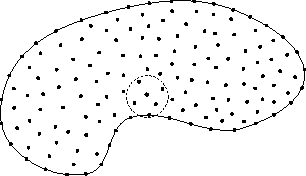
\includegraphics[width=0.7\textwidth]{images/domain_theoretical.pdf}
  \caption{Primer domene z diskretizirano notranjostjo in robom skupaj z izbrano
  točko in njeno soseščino.}
  \label{fig:domain-example}
\end{figure}

V okolici točke $p$ aproksimirajmo $u$ z elementi iz nekega končno
dimenzionalnega prostora funkcij $\B = \Lin\{b_1, \dots, b_m\}$.
Funkcijam $b_i\colon \R^d \to \R$ pravimo \emph{bazne funkcije},
številu $m$ pa moč baze. Aproksimacijo za $\uh$ za $u$ lahko torej zapišemo kot
\[
  u \approx \uh = \sum_{i=1}^m \alpha_i b_i = \b{b}^\T \b{\alpha},
\]
pri čemer smo z $\b{\alpha} = (\alpha_i)_{i=1}^m$ označili vektor neznanih
koeficientov in $\b{b} = (b_i)_{i=1}^m$ vektor baznih funkcij.

Če bi poznali vrednosti $u(x_i)$ za $i \in I(p)$, potem bi lahko aproksimiranko
$\uh$ izračunali po metodi najmanjših kvadratov. Ker pa teh vrednosti ne
poznamo, uvedimo spremenljivke $u_i$ za vsako točko v domeni, ki nam bodo
predstavljale neznane prave vrednosti in nadaljujmo
s simbolnim računanjem. Za funkcijo $\uh$ zahtevamo, da aproksimira $u$ v smislu
utežene diskretne 2-norme, torej da minimizira
\begin{align*}
  \|u-\uh\|_{2,N(p),\b{w}} &= \sum_{i\in I(p)} w(p-x_i) (u_i - \uh(x_i))^2
\end{align*}
kar je utežena vsota kvadratov odstopanj od pravih vrednosti. Pri tem je
$w\colon\R^d\to\R$ nenegativna funkcija, ki jo imenujemo \emph{utež}, $\b{w}$ pa
je vektor sestavljen iz vrednosti te funkcije v točkah v soseščini.

Matrično lahko zapišemo sistem enačb, ki po vrsticah
postavlja našo zahtevo $\hat{u}(x_j) = u_j$, za vsak $j \in I(p)$:
\begin{equation}
\begin{bmatrix}
  b_1(x_{i_1}) & \cdots & b_m(x_{i_1}) \\
  \vdots & \ddots & \vdots   \\
  b_1(x_{i_n}) & \cdots & b_m(x_{i_n})
\end{bmatrix}
\begin{bmatrix}
  \alpha_1 \\ \vdots \\ \alpha_m
\end{bmatrix}
=
\begin{bmatrix}
  u_{i_1} \\ \vdots \\ u_{i_n}
\end{bmatrix}.
  \label{eq:shape-system}
\end{equation}
Na krajše sistem zapišemo kot $B\b{\alpha} = \b{\tilde{u}}$. Odvisno od
$n$, $m$, $b_i$ in uteži $w$ je ta sistem lahko poddoločen, predoločen ali
običajen. V vsakem primeru lahko minimiziranje utežene napake prevedemo na
minimiziranje diskretne 2-norme $\|WB\b{\alpha}-W\b{\tilde{u}}\|_{2,N(p)}$, kjer je $W$
diagonalna matrika iz korenov uteži za posamezne točke, $W =
\diag(\sqrt{w(x_{i_1}-p)}, \dots, \sqrt{w(x_{i_n}-p)})$. Tak sistem pa lahko ne
glede na njegovo določenost v rešimo s pomočjo Moore-Penroseovega
psevdoinverza, ki ga lahko izračunamo s pomočjo singularnega razcepa matrike
$WB$.
Tako lahko izrazimo \[ \b{\alpha} = (WB)^{+}W\b{\tilde u}, \]
kjer $+$ označuje Moore-Penroseov psevdoinverz.

To lahko vstavimo nazaj v izraz za $\hat{u}$ in dobimo
\[
  \hat{u} = \b{b}^\T\b{\alpha} = \b{b}^\T(WB)^{+}W\b{\tilde{u}}.
\]
Sedaj lahko za izbrano točko $p$ izračunamo
\[
  \hat{u}(p) = \underbrace{\b{b}(p)^\T(WB)^{+}W}_{\b\phi_p}\b{\tilde{u}}.
\]
Izračunljivi kos $\b\phi_p$ je v praksi vrstica velikosti $n$, matematično pa je
linearen funkcional $\b\phi_p \in (\R^n)^\ast$, ki naboru funkcijskih vrednosti v
soseščini $N(p)$ priredi aproksimacijo za funkcijsko vrednost v točki $p$.

Podobno kot pri deljenih diferencah odvode funkcije $u$ aproksimiramo z odvodi
aproksimacijskega polinoma skozi točke v soseščini, bomo tudi v našem primeru
aproksimirali odvode funkcije $u$ z odvodi $\uh$,
\[
  (\L u)(p) \approx (\L \uh)(p) = (\L\b{b})(p)^\T(WB)^{+}W \b{\tilde{u}}
\]
od koder kot prej definiramo
\begin{equation}
  \b\phi_{\L,p} = (\L\b{b})(p)^\T(WB)^{+}W
  \label{eq:shape-definition}
\end{equation}
Funkcional $\b\phi_{\L,p}$ je aproksimacija operatorja $\L$ v točki $p$.
Pogosto se ga imenuje tudi \emph{funkcija oblike}~\ang{shape function}, saj v
sebi nosi podatke o lokalni obliki domene in izboru okoliških točk, ter seveda o
obnašanju $\L$ v tej okolici. Tudi če funkcijskih vrednosti $\b{\tilde{u}}$ v
okolici $p$ ne poznamo, lahko $\b\phi_{\L, p}$ izračunamo in kasneje samo s
skalarnim produktom dobimo aproksimacijo za $(\L u)(p)$. Lahko pa to izkoristimo
za zapis linearne enačbe
\[
  \b\phi_{\L,p} \cdot \b{\tilde{u}} = f(p),
\]
ki je direktna aproksimacija diferencialne enačbe~\eqref{eq:general-problem} v točki
$p$,
\[
  (\L u)(p) = f(p).
\]
To lahko sedaj storimo za vsako diskretizacijsko točko $x_i$ v domeni in
dobimo sistem enačb
\begin{align*}
  \b\phi_{\L,x_i} \cdot \b{\tilde{u}} &= f(x_i), \text{ za vsak $i$, tak da je $x_i \in \Omega$ } \\
  \b\phi_{\Rc,x_i} \cdot \b{\tilde{u}} &= g(x_i), \text{ za vsak $i$, tak da je $x_i \in \partial\Omega$.}
\end{align*}
Te enačbe lahko zapišemo v matrični sistem
\begin{equation}
  A\b{u} = \b{f},
  \label{eq:discretized-system}
\end{equation}
kjer ima matrika $A$ v vrsticah zapisane funkcionale $\b\phi_{\L,x_i}$, tako da so
neničelni elementi na tistih mestih, ki se pomnožijo z neznankami, ki ustrezajo
sosedom $x_i$. Natančneje, elementi matrike $A$ so
\begin{align*}
  A(k, i_j) &= \b\phi_{\L,p}(j), \text{ za vsak $k$, tak da je $x_k \in \Omega$
  in za vsak $i_j \in \I(x_k)$,} \\
  A(k, i_j) &= \b\phi_{\Rc,p}(j), \text{ za vsak $k$, tak da je $x_k \in
  \partial\Omega$ in za vsak $i_j \in \I(x_k)$.}
\end{align*}
Razumljivejša je morda kar Matlab-ova notacija
\[
A(k, I(x_k)) = \begin{cases}
    \b\phi_{\L, p} & x_k \in \Omega \\
    \b\phi_{\Rc, p} & x_k \in \partial\Omega \\
  \end{cases}, \text{ za $k = 1, \ldots, N$}.
\]
Vektor $\b{u} = (u_i)_{i=1}^N$ je vektor neznanih funkcijskih vrednosti, ki ga
iščemo, v vektorju $\b{f}$ pa so zapisani robni pogoji
\[
  \b f(k) = \begin{cases}
    f(x_k) & x_k \in \Omega \\
    g(x_k) & x_k \in \partial\Omega \\
  \end{cases}, \text{ za $k = 1, \ldots, N$}.
\]
Vidimo, da je matrika $A$ razpršena. Sama je dimenzij $N\times N$,
v vsaki vrstici pa ima največ $n$ neničelnih
elementov, torej je skupno število neničelnih elementov
\[
  \nnz(A) \leq nN.
\]
Enakost je lahko dosežena, lahko pa je tudi stroga, saj so kakšni koeficienti v $\phi_{\L,x_i}$ lahko
tudi 0, kot se to zgodi pri Dirichletovih robnih pogojih.

Sistem~\eqref{eq:discretized-system} nato rešimo in za aproksimacijo $u(x_i)$
vzamemo $u(x_i) \approx u_i$.

\subsection{Posebni primeri}
\label{sec:posebni-primeri}
Metoda iz razdelka~\ref{sec:splosna-izpeljava} je formulirana precej splošno, in
v posebnih primerih lahko prepoznamo druge znane metode. Za začetek pokažimo
enostavno trditev, ki bo metodo v določenih primerih poenostavila.
\begin{trditev}
  \label{trd:weight-independence}
  Če je $m = n$ in je matrika $B$ iz sistema~\eqref{eq:shape-system} obrnljiva,
  potem je izbira uteži nepomembna.
\end{trditev}
\proof
Spomnimo se, da je \[
  \b\phi = (\L\b{b})(p)^\T(WB)^{+}W.
\]
Matrika $W$ je diagonalna s sami pozitivnimi števili na diagonali in je torej
obrnljiva. Po predpostavki je obrnljiva tudi matrika $B$, torej je obrnljiv tudi
produkt $WB$ in velja
\[
  (WB)^+ = (WB)^{-1} = B^{-1}W^{-1}.
\]
Od tod sledi, da je
\[
  \b\phi = (\L\b{b})(p)^\T B^{-1} W^{-1} W = (\L\b{b})(p)^\T B^{-1},
\]
kar je neodvisno od $W$.
\endproof
\begin{opomba}
  Čeprav trditev~\ref{trd:weight-independence} velja v eksaktni aritmetiki v
  praksi ne velja nujno. Če so izbrane uteži zelo majhne ali zelo različnih
  velikosti lahko to povzroči nepotrebne numerične nestabilnosti.

  V praksi trditev kljub temu enostavno pomeni, da če izberemo toliko baznih
  funkcij kot imamo sosedov, je izbira uteži nepomembna.
\end{opomba}

Že v primeru~\ref{prim:fdm} smo videli, da se za Laplaceev robni problem na
intervalu naša metoda ujema z metodo končnih diferenc. Pokažimo to tudi v
primer dvodimenzionalne Poissonove enačbe.

\begin{trditev}
  \label{trd:eq-to-fdm}
  Metoda iz razdelka~\ref{sec:splosna-izpeljava} se za reševanje Poissonove
  enačbe na enakomerni pravokotni mreži z razmakom $h$ ujema z metodo končnih
  diferenc, če vzamemo $\b{b} = \{1, x, y, x^2, y^2\}$, $w \equiv 1$ in
  $n=5$.
\end{trditev}
\proof
Kot ponavadi označimo točke na mreži s koordinatami $(x_i, y_j)$, tako da je
$x_{i+1} = x_i + h$ in $y_{j+1} = y_j + h$.
Pokazati moramo, da se funkcija oblike v vsaki točki $x$ ujema z aproksimacijo
končnih diferenc,
ki pravi
\[
  (\triangle u)(x_i, y_j) = \frac{u_{i+1,j} + u_{i, j+1} + u_{i-1,j} + u_{i, j-1} -
  4u_{i,j}}{h^2},
\]
pri čemer spremenljivka $u_{i, j}$ pripada koordinati $(x_i, y_j)$. Če se
aproksimaciji Laplaceovega operatorja ujemata, potem se ujemati tudi
aproksimaciji rešitve, saj sistem pri obeh metodah gradimo na enak način.
Ker je operator krajevno neodvisen so tudi funkcije oblik odvisne samo od
medsebojne lege točk in torej lahko brez škode
za splošnost predpostavimo, da računamo funkcijo oblike za točko
$p = (0, 0)$. Najbližjih $n$ sosedov je tako $N(p) = \{(0, 0), (0, h), (0, -h),
(h, 0), (-h, 0)\}$. Matrika $B = [b_j(x_i)]$ iz sistema~\eqref{eq:shape-system},
ki ima po stolpic evalvirane bazne funkcije v vseh sosedih je
\[
  B =
  \begin{bmatrix}
    1 & 0 & 0 & 0 & 0 \\
    1 & 0 & -h & 0 & h^2 \\
    1 & 0 & h & 0 & h^2 \\
    1 & h & 0 & h^2 & 0 \\
    1 & -h & 0 & h^2 & 0 \\
  \end{bmatrix}
\]
in njen psevdoinverz je
\[
  B^+ = B^{-1} =
  \begin{bmatrix}
     1 & 0 & 0 & 0 & 0 \\
 0 & 0 & 0 & \frac{1}{2 h} & -\frac{1}{2 h} \\
 0 & -\frac{1}{2 h} & \frac{1}{2 h} & 0 & 0 \\
 -\frac{1}{h^2} & 0 & 0 & \frac{1}{2 h^2} & \frac{1}{2 h^2} \\
 -\frac{1}{h^2} & \frac{1}{2 h^2} & \frac{1}{2 h^2} & 0 & 0 \\
  \end{bmatrix}.
\]
Pri tem smo že upoštevali $w \equiv 1$.
Vektor vrednosti operatorja na baznih funkcijah je
\[
  (\triangle \b{b})(p) =
\begin{bmatrix}
  0 & 0 & 0 & 2 & 2
\end{bmatrix}^\T.
\]
Od tod dobimo po zvezi~\eqref{eq:shape-definition}
\[
  \b\phi = (\triangle \b b)(p)^\T B^{+} =
  \begin{bmatrix}
    -\frac{4}{h^2} & \frac{1}{h^2} & \frac{1}{h^2} & \frac{1}{h^2} &
    \frac{1}{h^2}
  \end{bmatrix},
\]
kar je ravno iskana aproksimacija.
\endproof
\begin{opomba}
  Metodo za izračun funkcije oblike je zelo elegantno implementirati v
  Mathematici, kar olajša simbolno raziskovanje takih aproksimacij. Zgornje matrike so
  bile izračunane s programa~\ref{prog:shape-mathematica}.

  \begin{listing}[!h]
    \vspace{-1ex}
  \begin{minted}[frame=lines,linenos,fontsize=\scriptsize]{wolfram}
(* podatki *)
p = {0, 0};
sosedi = {p, {0, -h}, {0, h}, {h, 0}, {-h, 0}};
bazne = {(1 &), (#1 &), (#2 &), (#1^2 &), (#2^2 &)};
operator = Function[f, Function[{x, y}, Derivative[2, 0][f][x, y] + Derivative[0, 2][f][x, y]]];
(* izračun *)
B = Table[Table[b @@ s, {b, bazne}], {s, sosedi}];
Lb = Table[operator[b] @@ p, {b, bazne}];
phi = Lb.PseudoInverse[B] // Simplify
  \end{minted}
  \vspace{-3ex}
  \caption{Računanje funkcij oblike na pravokotni mreži.}
  \label{prog:shape-mathematica}
  \end{listing}
\end{opomba}
\begin{opomba}
  \label{op:fdm-9}
  Tudi če izberemo $n=9$ in $\b b = \{1, x, x^2, y, xy, xy^2, y^2, y^2 x, y^2
  x^2 \}$, dobimo enako aproksimacijo kot v trditvi~\ref{trd:eq-to-fdm}, le da
  uporabimo več sosedov. Če jih uredimo po oddaljenosti od $(0, 0)$ dobimo
  aproksimacijo
  \[
    \b\phi =  \begin{bmatrix}
    -\frac{4}{h^2} & \frac{1}{h^2} & \frac{1}{h^2} & \frac{1}{h^2} &
    \frac{1}{h^2} & 0 & 0 & 0 & 0
  \end{bmatrix}.
\]
 Če pa bi izbrali $n=25$ točk in bazne funkcije $\b b = \{x^iy^j, 0 \leq i, j
 \leq 4 \}$, potem bi dobili aproksimacijo četrtega reda.
\end{opomba}
\begin{primer}
  Naredimo še en primer, kjer za bazne funkcije vzamemo monome. Vzemimo tokrat
  $n = 9$ in za bazne funkcije vse monome skupne stopnje manj kot 3, torej $\b b = \{1,
  x, y, x^2, y^2, xy\}$. V tem primeru je matrika $B$ velikosti $9\times 6$ in
  s pomočjo programa~\ref{prog:shape-mathematica} dobimo
  \[
    \b\phi =
    \begin{bmatrix}
-\frac{4}{3 h^2} & -\frac{1}{3 h^2} & -\frac{1}{3 h^2} & -\frac{1}{3 h^2} &
-\frac{1}{3 h^2} & \frac{2}{3 h^2} & \frac{2}{3 h^2} & \frac{2}{3 h^2} &
\frac{2}{3 h^2}
    \end{bmatrix}.
  \]
  Vidimo, da tokrat v aproksimaciji upoštevamo vseh 9 sosedov, z razliko od
  aproksimacije v opombi~\ref{op:fdm-9}. Naravno sledi vprašanje, ali je ta
  aproksimacija kaj slabša, morda drugačnega reda? Izkaže se da ne, saj z
  razvojem aproksimacij v Taylorjevo vrsto dobimo
  \scriptsize
  \begin{align*}
    &\frac{-4 u(0, 0) + u(0, h) + u(0, -h) + u(h, 0) + u(-h, 0)}{h^2} = \\
    & \qquad = \triangle u + \frac{h^2}{12}\left(\dpar{^4u}{x^4}(0,0) +
  \dpar{^4u}{y^4}(0, 0)\right) + O(h^4) \\
    &\frac{-4 u(0, 0) - u(0, h) - u(0, -h) - u(h, 0) - u(-h, 0)
    + 2u(h, h) + 2u(h, -h) + 2u(-h, h) + 2u(-h, -h)}{3h^2} = \\
    & \qquad =
    \triangle u + \frac{h^2}{12}\left(\dpar{^4u}{x^4}(0,0) + \dpar{^4u}{x^2y^2}(0,0) +
    \dpar{^4u}{y^4}(0, 0)\right) + O(h^4).
  \end{align*}
  \normalsize
  Obe aproksimaciji sta torej drugega reda, razlikujeta se le pri izražavi
  napake.
\end{primer}

\begin{primer}
\label{prim:rbf}
Poglejmo še, kaj se zgodi, če za bazne funkcije vzamemo radialne bazne funkcije.
V tem primeru je smiselno vzeti $n = m$, torej postavimo po eno radialno funkcijo
na vsakega izmed sosedov. Opisana metoda tako postane kolokacijska metoda z
lokalnimi radialnimi baznimi funkcijami \ang{local radial basis function
collocation method}.

Če za $n = 9$ sosedov točke $(0, 0)$ izberemo točke \[ N(p) = \{
  (0, 0), (0, h), (0, -h), (h, 0), (-h, 0), (h, h), (h, -h), (-h, h), (-h, -h)
\} \] in za $\b b$ vzamemo \[ \b b = \{ x\mapsto \exp((x-c)^2/\sigma^2); c \in N(p)
\}, \]
potem zopet s
pomočjo programa~\ref{prog:shape-mathematica} izračunamo aproksimacijo
\small
\[
  \b\phi =\frac{4}{(e^{\frac{2 h^2}{\sigma^2 }}-1)^2 \sigma^4}
\begin{bmatrix}
  (e^{\frac{2 h^2}{\sigma^2 }}-1)^2 -4h^2 e^{\frac{2 h^2}{\sigma^2 }} &
   h^2e^{\frac{h^2}{\sigma^2 }} & h^2e^{\frac{h^2}{\sigma^2 }} &
   h^2e^{\frac{h^2}{\sigma^2 }} & h^2e^{\frac{h^2}{\sigma^2 }} & 0 & 0 & 0 & 0
 \end{bmatrix}.
\]
\normalsize
Tokrat vidimo, da se precej razlikuje od aproksimacije s končnimi diferencami.
Toda, še vedno je drugega reda, saj za napako velja
\[
  \b \phi\cdot \b{\tilde{u}} - \triangle u(0, 0) =
  h^2\left(\frac{2u(0,0)}{\sigma^2} - \frac{\triangle u(0,0)}{\sigma^2} +
  \frac{1}{12}\left( \dpar{^4u}{x^4}(0,0) + \dpar{^4u}{y^4}(0, 0) \right)\right)
  + O(h^4).
\]
\end{primer}

\subsection{Algoritem}
V izpeljavi metode v razdelku~\ref{sec:splosna-izpeljava} je veliko detajlov
ostalo neizdelanih, kot na primer, kako diskretiziramo domeno ali kako poiščemo
sosede. Ti detajli so opisani v naslednjih podrazdelkih, celotno metodo pa podajamo v
psevdokodi kot algoritem~\ref{alg:metoda}.

\begin{algorithm}[!ht]
  \caption{Brezmrežna metoda za reševanje PDE iz
  razdelka~\ref{sec:splosna-izpeljava}.}
  \textbf{Vhod:} Parcialna diferencialna enačba, kot opisana
  v~\eqref{eq:general-problem}. Parametri metode: \\
  \begin{tabular}{llll}
    \algorithmlist & $N$     & \ldots & celotno število diskretizacijskih točk    \\
    \algorithmlist & $Q$     & \ldots & število diskretizacijskih točk v
    notranjosti $\Omega$ \\
    \algorithmlist & $n$     & \ldots & število sosedov, ki jih ima vsaka točka   \\
    \algorithmlist & $m$     & \ldots & število baznih funkcij                    \\
    \algorithmlist & $b$ & \ldots & seznam baznih funkcij dolžine $m$         \\
    \algorithmlist & $w$     & \ldots & utež
  \end{tabular} \\
  \textbf{Izhod:} Skalarno polje $u$, ki aproksimira rešitev
  enačbe~\eqref{eq:general-problem}.
  \label{alg:metoda}
  \begin{algorithmic}[1]
    \Function{reši}{$\Omega, \L, f, \Rc, g, N, Q, n, m, b, w$}
    \State $x \gets \textsc{diskretiziraj}(\Omega, N, Q)$
    \Comment{$x$ postane seznam $N$ točk, brez škode za splošnost naj leži prvih
    $Q$ točk v $\Omega$ in preostalih $N-Q$ na $\partial \Omega$.}
    \State $s \gets \textsc{sosedi}(x, n)$ \label{line:kdtree}
    \Comment{$s$ je seznam dolžine $N$, pri čemer je $s[i]$ seznam indeksov
    elementov v $x$, ki so sosedi $x[i]$, vključno z $i$.}
    \State $\phi \gets$ prazen seznam dolžine $N$.
    \For{i}{1}{Q} \Comment{Izračunamo funkcije oblik v notranjosti.}
    \State $\phi[i] \gets$ \textsc{funkcijaOblike}$(\L, x[i], x, s[i], n, m, b, w)$
    \Comment{Glej algoritem~\ref{alg:shape-function}.}
    \EndFor
    \For{i}{Q+1}{N} \Comment{Izračunamo funkcije oblik na robu.}
    \State $\phi[i] \gets$ \textsc{funkcijaOblike}$(\Rc, x[i], x, s[i], n, m, b,
    w)$
    \Comment{Glej algoritem~\ref{alg:shape-function}.}
    \EndFor
    \State $A \gets$ prazna razpršena $N\times N$ matrika
    \For{i}{1}{N} \Comment{Aproksimiramo enačbo.}
    \For{j}{1}{n}
    \State $A[i, s[j]] \gets \phi[i][j]$
    \EndFor
    \EndFor
    \State $r \gets$ prazen vektor dolžine $N$
    \For{i}{1}{Q} \Comment{Izračunamo desno stran v notranjosti.}
    \State $r[i] \gets f(x[i])$
    \EndFor
    \For{i}{Q+1}{N} \Comment{Izračunamo robne pogoje.}
    \State $r[i] \gets g(x[i])$
    \EndFor
    \State $u \gets$ \textsc{rešiRazpršenSistem}$(A, r)$
    \State \Return $u$
    \EndFunction
  \end{algorithmic}
\end{algorithm}

\begin{algorithm}[!ht]
  \caption{Izračun funkcije oblike.}
  \textbf{Vhod:} Parametri metode: \\
  \begin{tabular}{llll}
    \algorithmlist & $\L$    & \ldots & parcialen diferencialen operator \\
    \algorithmlist & $p$     & \ldots & točka, v kateri aproksimiramo operator \\
    \algorithmlist & $x$     & \ldots & seznam diskretizacijskih točk \\
    \algorithmlist & $I$     & \ldots & množica indeksov točk v soseščini $p$ \\
    \algorithmlist & $n$     & \ldots & število sosedov, ki jih ima vsaka točka   \\
    \algorithmlist & $m$     & \ldots & število baznih funkcij                    \\
    \algorithmlist & $b$     & \ldots & seznam baznih funkcij dolžine $m$         \\
    \algorithmlist & $w$     & \ldots & utež
  \end{tabular} \\
  \textbf{Izhod:} Funkcional, ki aproksimira operator $\L$ v točki $p$.
  \label{alg:shape-function}
  \begin{algorithmic}[1]
    \Function{funkcijaOblike}{$\L, p, x, I, n, m, b, w$}
    \State $W \gets$ prazen vektor dolžine $n$
    \For{i}{1}{n}
    \State $W[i] \gets \sqrt{w(x[I[i]]-p)}$
    \EndFor
    \State $B \gets $ prazna matrika velikosti $n \times m$
    \For{i}{1}{n}
    \For{j}{1}{m}
    \State $B[i, j] \gets W[i] \cdot  b[j](x[I[i]])$
    \EndFor
    \EndFor
    \State $\ell \gets$ prazen vektor dolžine $m$
    \For{j}{1}{m}
    \State $\ell[j] \gets (\L (b[j]))(p)$
    \EndFor
    \State $\phi \gets (\ell \cdot \textsc{pinv}(B)) \odot W$
    \Comment{Direktna analogija enačbe~\eqref{eq:shape-definition}, $\odot$
  označuje}
    \State \Return $\phi$
  \Comment{Hadamardov produkt.}
    \EndFunction
  \end{algorithmic}
\end{algorithm}

\subsubsection{Diskretizacija}
Splošno $d$-dimenzionalno domeno $\Omega$ je težko dobro diskretizirati.
Želimo si, da bi bile točke v domeni čim bolj enakomerno razporejene, saj to
pomeni, da smo dobro popisali celotno področje in upamo, da s tem tudi obnašanje
funkcije $u$, hrakti pa si zaradi numerične stabilnosti ne želimo, da bi bile
točke preveč skupaj. Uvedimo dve količini, ki nam merita ti dve lastnosti.
Za dano domeno $\Omega$ in množico točk $X$ definirajmo
\begin{align}
  h_\Omega(X) &= \max_{p \in \Omega} \min_{x \in X} \|p - x\| \\
  \label{eq:def-hs}
  S(X) &= \min_{\substack{x, y \in \Omega \\ x \neq y}} \|x-y\| \nonumber
\end{align}
Količina $h$ pove, da ne glede na to, kje v domeni smo, imamo na razdalji manj ali enako $h$
vsaj eno diskretizacijsko točko. Količina $S$ pa pove, kako blizu so si
diskretizacijske točke med seboj. Dobra diskretizacija želi maksimizirati $S$ in
minimizirati~$h$.

Algoritmi za diskretizacijo odvisni od načina, kako podamo domeno.
V našem se izkaže, da je za trenutne potrebe dovolj, da podpiramo
kvadre in krogle do vključno treh dimenzij, kot tudi unije in razlike
osnovnih oblik.

Tako lahko za diskretizacijo kvadra uporabimo kar enakomerno diskretizacijo.
Prav tako ni težko ugotoviti, kdaj so točke na robu. Za čimbolj enakomerno
diskretizacijo notranjosti kroga ali površine sfere
lahko uporabimo npr.~Fibonaccijevo mrežo, kot predlagano
v~\cite{hannay2004fibonacci} ali~v~\cite{gonzalez2010measurement}.
Pri razlikah domen preprosto izbrišemo točke, ki so padle izven domene,
pri unijah pa naredimo tudi unijo diskretizacij. Pri tem lahko potem naredimo še
en korak in pobrišemo ven kakšno izmed točk, ki so si preblizu skupaj.
Primeri domen in njihovih diskretizacij dobljenih na ta način so prikazani na sliki~\ref{fig:domains}.
\begin{figure}[!ht]
  \centering
  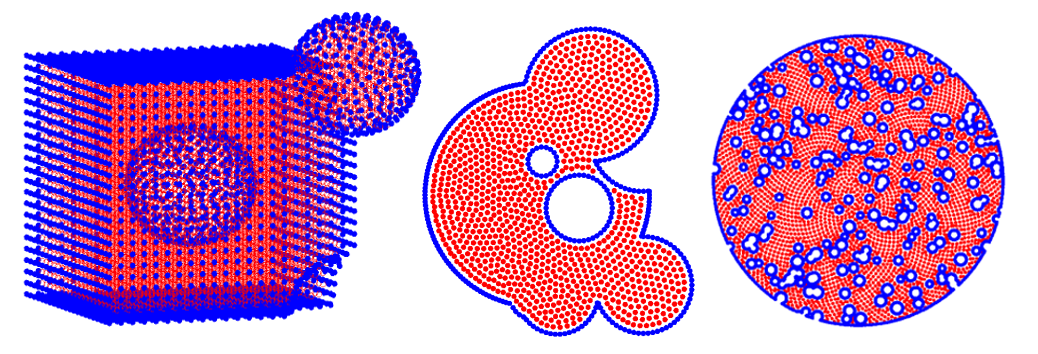
\includegraphics[width=\textwidth]{images/domains_generated.png}
  \caption{Primeri domen in njihovih diskretizacij.}
  \label{fig:domains}
\end{figure}

Pri enakomerni diskretizaciji smo močno uporabili naše znanje o domeni in njeni
obliki. Lahko pa, da tega nimamo na voljo in želimo splošnejši algoritem, ki
potrebuje npr.~samo karakteristično funkcijo domene in njene meje, torej, kakšen
kvader, ki našo domeno vsebuje.
V tem primeru lahko vzamemo enakomerno diskretizacijo kvadra in odstranimo vse
točke, ki niso v domeni, vendar je tu težko kontrolirati število točk.
Druga metoda je, da naključno izbiramo točke v kvadru, in sprejmemo tiste, ki
pristanejo v notranjosti. Še boljšo diskretizacijo dobimo, če namesto
psevdonaključnih števil uporabimo kvazinaključna števila, ki imajo manjšo
diskrepanco. Več o tem si bralec lahko prebere v~\cite{morokoff1994quasi}.

Kljub njihovi splošnosti so naključne diskretizacije precej slabe, kot na primer
naključna diskretizacija kroga na sliki~\ref{fig:relax-circle} (levo).
Pri tem, da bi točke v domeni porazdelili čimbolj enakomerno, si lahko pomagamo
s preprostim iterativnim postopkom, za katerega se izkaže, da v praksi dobro
deluje. Navdih jemljemo iz fizike in si zamislimo, da je vsaka točka naboj, ki
se odbija od sosednjih točk in pustimo fiziki, da opravi svoje delo.
Na vsako točko tako deluje neka sila, ki jo sili
stran od drugih točk, v prazen prostor. Točko lahko malo premaknemo v smeri
sile, ponovno izračunamo medsebojne sile in postopek ponavljamo. Pri tem točkam
na robu ne dovolimo premikanja in če kakšna točka iz notranjosti zleze iz
domene, jo postavimo na naključno mesto nazaj v domeno. Zapis zgornjega postopka
je v psevdokodi je podan kot algoritem~\ref{alg:relax}. Postopku se kdaj reče
tudi \emph{sprostitev} \ang{relaxation} domene, kajti na začetku so med točkami
napetosti, ki jih s premikanjem poskušajo minimizirati. Rezultati na primeru
izboljšanja naključne diskretizacije kroga so podani na
sliki~\ref{fig:relax-circle}.

\begin{algorithm}[!ht]
  \caption{Algoritem za izboljšanje kvalitete diskretizacije domene.}
  \textbf{Vhod:} Parametri metode: \\
  \begin{tabular}{llll}
    \algorithmlist & $\Omega$  & \ldots & domena \\
    \algorithmlist & $N$       & \ldots & število diskretizacijskih točk \\
    \algorithmlist & $Q$       & \ldots & število diskretizacijskih točk v
    notranjosti $\Omega$ \\
    \algorithmlist & $X$       & \ldots & seznam diskretizacijskih točk, prvih $Q$
    je v notranjosti. \\
    \algorithmlist & $I$       & \ldots & število iteracij \\
    \algorithmlist & $s$       & \ldots & število sosedov, ki jih upoštevamo pri delovanju sile \\
    \algorithmlist & $F_0$     & \ldots & delež sile, ki vpliva na premik \\
    \algorithmlist & $\alpha$  & \ldots & eksponent v sili                \\
  \end{tabular} \\
  \textbf{Izhod:} Nov seznam diskretizacijskih točk.
  \label{alg:relax}
  \begin{algorithmic}[1]
    \Function{izboljšaj}{$\Omega, N, Q, X, I, s, F_0, \alpha$}
    \State $r_\chi \gets \left( \frac{\textsc{volumen}(\Omega)}{N}
    \right)^{\frac{1}{\textsc{dimenzija}(\Omega)}}$ \Comment{Približek povprečne
    razdalje med točkami}. \label{line:chd}
    \For{i}{1}{I}
    \For{j}{1}{Q}
    \State $\vec{F} \gets \vec{0}$
    \ForEach{y}{\{najbližjih $s$ sosedov $X[i]$\}} \label{line:closest}
    \State $\vec{r} \gets \frac{X[i] - y}{r_\chi}$ \Comment{Brezdimenzijski vektor
    razdalje.}
    \State $\vec{F} \gets \vec{F} + \frac{\vec{r}}{\|\vec{r}\|^\alpha}$
    \EndFor
    \State $X[i] \gets X[i] + F_0 \vec{F}$.
    \If{$X[i] \notin \Omega$}
    \State $X[i] \gets $ naključna pozicija znotraj $\Omega$
    \EndIf
    \EndFor
    \EndFor
    \State \Return $X$
    \EndFunction
  \end{algorithmic}
\end{algorithm}

\begin{figure}[!ht]
  \centering
  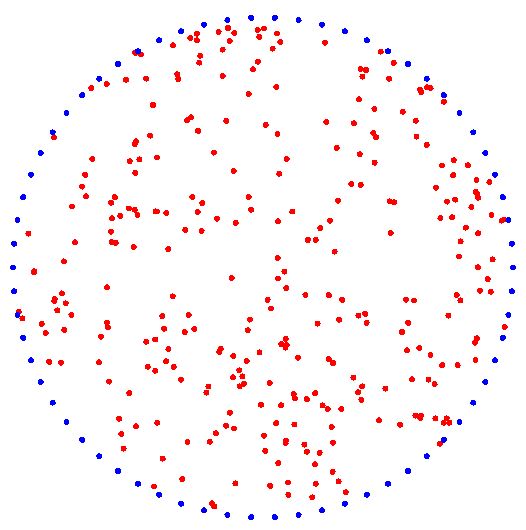
\includegraphics[width=0.3\textwidth]{images/domain_circle.png}
  \hspace{1em}
  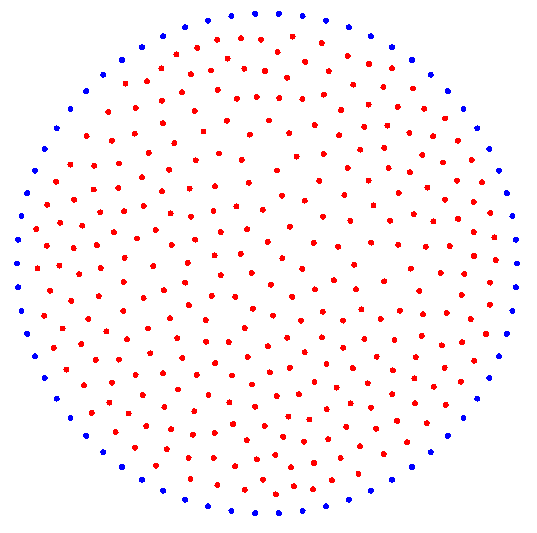
\includegraphics[width=0.3\textwidth]{images/domain_circle_relaxed.png}
  \caption{Primerjava domene z naključno diskretizacijo (levo) in domene po
  izvedbi 10 iteracij algoritma~\ref{alg:relax} s parametri $F_0 = 10^{-2}$, $s
  = 6$, $\alpha = 3$ (desno).}
  \label{fig:relax-circle}
\end{figure}

Da algoritem izboljša kvaliteto aproksimacije se vidi tudi, če izračunamo
parametra $h$ in $S$. Pričakujemo, da se bo $S$ povečal, saj se točke, ki so
bolj skupaj, bolj odbijajo. Na sliki~\ref{fig:relax-hs} vidimo primerjavo med
kvaliteto diskretizacije s Fibonaccijevo mrežo in njeno 10-kratno izboljšavo.
Vidimo da se $h$ ni bistveno spremenil, le varianca se mu je malce povečala,
$S$ pa se je v povprečju precej izboljšal in izkazuje celo lepše obnašanje kot
prej.

\begin{figure}[ht]
  \centering
  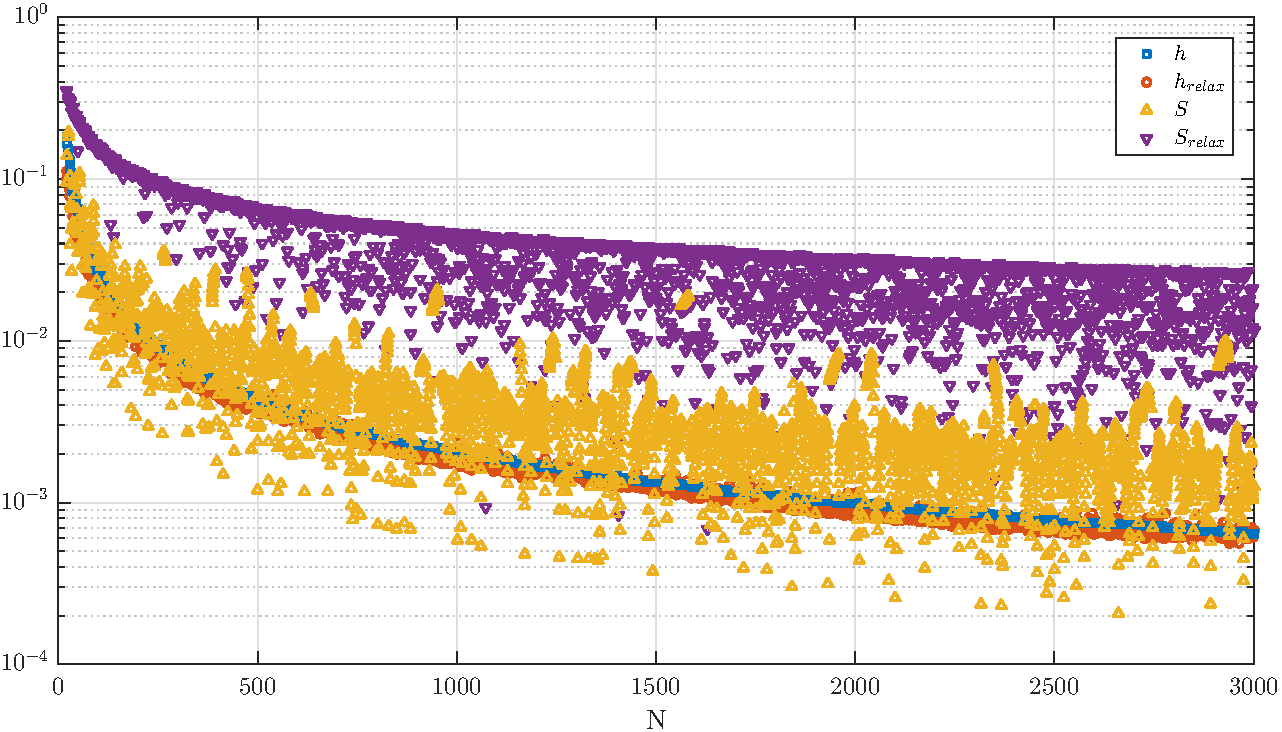
\includegraphics[width=0.8\textwidth]{images/relax_improvement.pdf}
  \caption{Sprememba $h$ in $S$ po 10 iteracijah algoritma~\ref{alg:relax} s
  parametri $F_0 = 10^{-2}$, $s = 6$, $\alpha = 3$ v enotskem dvodimenzionalnem
  krogu z začetno Fibonaccijevo mrežo v odvisnosti od $N$ z razmerjem robnih in
  notranjih točk $x : \frac{12}{\pi} \sqrt{x}$.}
  \label{fig:relax-hs}
\end{figure}


\subsubsection{Iskanje najbližjih sosedov}

Tako v algoritmu~\ref{alg:metoda} v vrstici~\ref{line:kdtree} kot v
algoritmu~\ref{alg:relax} v vrstici~\ref{line:closest} potrebujemo
najti nekaj najbližjih sosedov dane točke. Navadno za okolico izberemo kar
$n$ najbližjih sosedov v evklidski metriki, vendar bi lahko soseščino definirali
tudi drugače, na primer kot množico vozlišč, ki so oddaljeni manj kot neka
fiksna razdalja $R$.  Pri tem pristopu bi imeli manjšo kontrolo nad velikostjo
soseščine, zato izberemo prvega.

Problem iskanja najbližjih sosedov \ang{nearest neighbour search} je znana in
dobro raziskana tema z razvitimi veliko podatkovnimi strukturami, ki podpirajo
grajenje, iskanje, vstavljanje in brisanje v logaritemskem času. Večina jih
temelji na delitvi prostora na različne hierarhično urejene podprostore, ki jih
potem hranimo v drevesni strukturi, kar nam omogoča logaritemski dostop. Med
bolj znanimi strukturami so \emph{$k$-d tree}~\cite{moore1991intoductory},
\emph{ball tree}~\cite{omohundro1989five} in \emph{cover
tree}~\cite{beygelzimer2006cover}. V članku~\cite{kibriya2007empirical} je
narejena empirična primerjava med zgornjimi tremi strukturami, ki pokaže, da
so v primeru nizkih dimenzij (kar gotovo vsebuje $d \leq 3$) najboljše obnese
\emph{$k$-d tree}. Poleg tega \emph{$k$-d tree} najboljše deluje tudi, ko imajo
točke, v katerih bomo iskali sosede podobno porazdelitev kot točke, iz katerih
smo naredili drevo, kar v našem primeru drži. Če vključimo še dejstvo, da je
\emph{$k$-d tree} tudi najpopularnejša rešitev za problem najbližjih sosedov
in ima na voljo veliko prosto dostopnih implementacij, je to dovolj argumentov,
da jo uporabimo tudi mi. Specifična uporabljena implementacija je predstavljena
v~\cite{mount1998ann}, ki za shrambo $N$ točk porabi $O(N)$ prostora in
odgovarja na poizvedbe o $n$ najbližjih sosedih v $O(n\log N)$ časa.
S pomočjo tega postane implementacija funkcije \textsc{sosedi} iz
algoritma~\ref{alg:metoda} trivialna, pri algoritmu~\ref{alg:relax} pa si na
vsaki iteraciji na novo zgradimo drevo in ga uporabimo za iskanje $s$ najbližjih
sosedov.

\subsubsection{Reševanje razpršenega sistema}
Za reševanje razpršenih sistemov poznamo veliko različnih metod, ki se v grobem
delijo na direktne (obsežno opisane v~\cite{davis2006direct}) in iterativne
(obsežno opisane v~\cite{saad2003iterative}).
Pri običajnih, polnih matrikah bi za reševanje splošnega sistema linearnih enačb
uporabili LU razcep in razcepili matriko $A$ kot $A = LU$. Toda, tudi če je
matrika $A$ razpršena, v splošnem $L$ in $U$ nista nujno in sta lahko celo
polni, kar povzroči, da nam zmanjka pomnilnika. Direktne metode, kot na primer
SuperLU~\cite{li2005overview} poskušajo z
preureditvijo stolpcev v razpršeni matriki $A$ minimizirati število novih
neničlenih elementov v matrikah $L$ in $U$. Po drugi strani iterativne metode
aproksimirajo pravilno rešitev sistema $Ax=b$ z zaporedjem približkov $\{x^{(r)}\}$,
ki naj bi konvergirali k $x$. Te metode običajno ne zahtevajo veliko pomnilnika,
je pa natančnost približka odvisna od števila porabljenih iteracij, tako da
moramo za višjo natančnost porabiti večje število računskih operacij.

Za metode iz numerične linearne algebre bomo uporabljali knjižnico
Eigen~\cite{eigenweb}, ki nudi elegantno in hitro delo z matrikami v C++.
Vgrajenih ima veliko direktnih in iterativnih metod za reševanje sistemov
linearnih
enačb.\footnote{\url{https://eigen.tuxfamily.org/dox/group__TopicSparseSystems.html}
  \newline
[obiskano 17.\ 6.\ 2017]}
Pri sistemih tipa~\eqref{eq:discretized-system} se je
v praksi najbolje obnesel BiCGSTAB~\cite{van1992bi} z
ILUT predpogojevanjem~\cite{saad1994ilut}. BiCGSTAB v primeru uporabe pravilne
shrambe matrike v pomnilniku podpira tudi paralelizacijo, poleg tega pa je
konvergenca v praksi dovolj hitra. Predpogojevanje z uporabo nepopolnega LU
razcepa z dvojnim pragom~\ang{dual threshold incomplete LU factorization (ILUT)}
omogoča natančnejšo kontrolo nad porabljenim spominom in hitrostjo konvergence z
uporabo dveh parametrov $p$ in $\tau$. Med $LU$ faktorizacijo izpustimo vsak
element, ki je manjši kot $\tau\cdot e$, kjer je $e$ povprečna absolutna
vrednosti elementov v trenutni vrstici. Nato obdržimo le največjih $f$ elementov
v matrikah $L$ in $U$, kjer je $p$ uporabljen kot razmerje med $f$ in začetnim
številom neničelnih elementov. V grobem nam tako parameter $p$ kontrolira
kolikokrat več spomina dovolimo za hranjenje predogojenke,
parameter $\tau$ pa, kako natančna bo LU faktorizacija.

\subsubsection{Časovna zahtevnost}
V tem razdelku analiziramo časovno zahtevnost metode. Predpostavili bomo, da so
vse evalvacije funkcij $f$, $g$, $w$ in $b_j$, $\L b_j$, $\Rc b_j$ izvedene v $O(1)$.
Prav tako bomo predpostavili, da je dimenzija problema majhna in konstantna in
ne bo nastopala v analizah.

\begin{trditev}
  Pričakovana časovna zahtevnost algoritma~\ref{alg:metoda} je
  \[ O(I N s \log^2 N + (N+n)\log N + m^2n N) + T,\] kjer je $T$ čas,
  porabljen za reševanje razpršenega sistema enačb.
\end{trditev}
\proof
Pri funkciji \textsc{diskretiziraj} predpostavimo, da uporabljamo enostavno
diskretizacijo, ki deluje v $O(N)$ časa, skupaj z $I$ iteracijami izboljšave
na $s$ sosedih, ki traja $O(I N s \log^2 N)$ časa, saj na vsaki iteraciji
konstruiramo drevo in iščemo $s$ sosedov vsake točke.

Izvajanje funkcije \textsc{sosedi} traja $O((N+n) \log N)$ časa za konstrukcijo
drevesa in iskanje sosedov.

Izvajanje funkcije \textsc{funkcijaOblike} traja po $O(n + nm + m + m^2n + nm +
n) = O(mn^2)$, kjer je prevladujoči faktor $O(m^2 n)$ rezultat računanja SVD
razcepa z dvostranskim Jacobi SVD razcepom iz knjižnice
Eigen.\footnote{\url{https://eigen.tuxfamily.org/dox/classEigen_1_1JacobiSVD.html}
[obiskano 16.\ 6.\ 2017]} Funkcija oblike se izračuna za vsako točko v domeni,
torej da del algoritma traja $O(m^2 n N)$ časa.

Pri sestavljanju razpršene matrike lahko v naprej rezerviramo prostor za $n$
elementov v vsaki vrstici, tako da nas sestavljanje matrike stane $O(nN)$ časa,
sestavljanje robnih pogojev pa $O(N)$ časa. Na koncu še rešimo razpršen sistem
linearnih enačb, kjer pa je čas zelo odvisen od problema, iteracijske metode in
predpogojenke.

Skupna časovna zahtevnost je tako $O(I N s \log^2 N + (N+n)\log N + m^2 N) + T$,
kjer je $T$ čas, porabljen za reševanje razpršenega sistema enačb.
\endproof

\subsubsection{Prostorska zahtevnost}
V tem razdelku analiziramo časovno zahtevnost metode. Podobno kot pri časovni
zahtevnosti bomo predpostavili, da so
vse evalvacije funkcij $f$, $g$, $w$ in $b_j$, $\L b_j$, $\Rc b_j$ izvedene v
$O(1)$ prostora.
Prav tako bomo predpostavili, da je dimenzija problema majhna in konstantna in
ne bo nastopala v analizah.

\begin{trditev}
  Prostorska zahtevnost algoritma~\ref{alg:metoda} je $O(nN) + P$, kjer je $P$
  prostor, ki ga potrebujemo, za reševanje sistema linearnih enačb.
\end{trditev}
\proof
Pri funkciji \textsc{diskretiziraj} potrebujemo $O(N)$ spomina za shrambo $N$
diskretizacijskih točk. Če izvajamo še dodatne izboljšave diskretizacije, nas to
stane $O(n)$ dodatnega prostora.

Izvajanje funkcije \textsc{sosedi} nas stane $O(N)$ prosta za hranjenje drevesa
in $O(nN)$ prosta za hranjenje indeksov $n$ sosedov.

Izvajanje funkcije \textsc{funkcijaOblike} nas stane $O(n+nm+m+n) = O(nm)$
prostora za vsak klic, za hrambo $N$ funkcij oblike pa potrebujemo $O(nN)$
prostora.

Razpršena matrika prav tako potrebuje $O(nN)$ prostora za neničelne elemente.
Nato moramo rešiti le še sistem linearnih enačb, kar po predpostavki stane $P$
prostora. Ker je $m = O(N)$ je prevladujoči faktor $O(nN)$ in skupna prostorska
zahtevnost je $O(nN) + P$.
\endproof

\subsection{Pogoste vrednosti parametrov}
Metoda je bila do sedaj formulirana zelo splošno, v praksi pa se uporablja nekaj
ustaljenih kombinacij. Kot bomo videli razdalje pogosto merimo v večkratnikih
$r_\chi$, kot na vrstici~\ref{line:chd} v algoritmu~\ref{alg:relax}.
\begin{definicija}
  Količino $r_\chi$ pripisano diskretizaciji $X$ domene $\Omega$, izračunano z \[
    r_\chi(\Omega, X) = \left( \frac{\textsc{volumen}(\Omega)}{|X|}
    \right)^\frac{1}{\textsc{dimenzija}(\Omega)}
  \]
  imenujemo \emph{karakteristična razdalja.}
\end{definicija}
Ideja definicije je, da $r_\chi$ predstavlja približno povprečno razdaljo med
diskretizacijskimi točkami, če bi bile razporejene enakomerno. Celoten volumen
domene razdelimo na $N = |X|$ delov, tako da vsaki točki pripada enak kos
volumna $v = \frac{\textsc{volumen}(\Omega)}{N}$. Če bi
bil ta kos neka hiperkocka v $d$ dimenzijah, potem je $\sqrt[d]{v}$ dolžina
njene stranice in to je ocena za medsebojno razdaljo med točkami.
V eni dimenziji $r_\chi$ do faktorja $\frac{N}{N-1}$ natančno ustreza razdalji
med enakomerno razporejenimi točkami.
Drugo pogosto merilo za lokalno razdaljo bo kar razdalja do najbližjega
(različnega) soseda, ki jo imenujmo $r_c$. To je težje izračunati, če nimamo že
zgrajenega drevesa, zato se ponavadi na enostavnejših primerih poslužujemo kar
$r_\chi$. Kadar pa to ni dobra aproksimacija razdalje med vozlišči za celo
domeno, kot na primer ob goščenju mreže, se poslužimo $r_c$.

Pogoste vrednosti za število sosedov so $n = 3, 5, 7$ v eni dimenziji, $n = 5,
9, 13, 25$ v dveh dimenzijah in $n = 7$ ali $27$ v treh dimenzijah. Za regularne
domene to simetrično izbere vozlišča pri neregularnih pa izbira $n$ ni tako
pomembna, dokler je dovolj visoka, da dobro popiše operator, ki ga aproksimiramo.
Višji $n$ ponavadi pomeni večjo stabilnost, morda višji red in počasnejše
izvajanje. V praksi izberemo najmanjši $n$, ki daje zadovoljive rezultate.

Za utež se pogosto uporablja konstanta $w\equiv1$, če ne želimo uteženih
najmanjših kvadratov, sicer pa pogosto vzamemo za utež Gaussovo funkcijo
\[
  w(x) = \exp\left(-\left(\frac{x}{\sigma_w}\right)^2 \right),
\]
kjer $\sigma_w$ imenujemo parameter oblike \ang{shape parameter} uteži.
Velja opozoriti, da je ta funkcija praktično nič, če smo več kot $3\sigma_w$
stran od središča ($w(3\sigma_w) \approx 0.0001234$). Če na primer izberemo
$\sigma_w = r_\chi$ se nam vsi sosedi, ki so dlje kot $r_\chi$ stran v
aproksimaciji ne upoštevajo, ne glede na to kako velik $n$ smo izbrali.
Ponavadi se za $\sigma_w$ začne izbirati vrednosti okoli $r_\chi$, je
pa potrebno optimalno vrednost določiti za vsak posamezen problem posebej.

Pogosta izbira baznih funkcij so prostori $\mathbb{P}_\ell$ monomov skupne
stopnje manj ali enako $\ell$. Pri tem moramo seveda paziti, da izberemo dovolj
visok $n$. Druga pogosta izbira je, da vzamemo $m = n$ in za bazne funkcije
izberemo radialne bazne funkcije s centri v sosedih.

\begin{definicija}
  Funkcija $\psi_c$ se imenuje radialna bazna funkcija s centrom v točki
  $c$,
  če je odvisna samo od razdalje do centra, torej \[
    \psi_c(x) = \tilde\psi(\|x - c\|),
  \]
  za vsak $x$ za neko funkcijo $\psi$. Kasneje kar identificiramo $\psi_c$
  in $\tilde\psi$ in pišemo $\psi_c = \psi_c(r)$.
\end{definicija}

V tabeli~\ref{tab:rbf} so naštete najpogostejše uporabljene radialne bazne funkcije, povzete
po~\cite[str.\ 5]{schaback1995error}.

\newcommand{\tc}[1]{\vspace{-25ex}\parbox{5.2cm}{#1}}
\begin{table}[!h]
  \begin{tabular}{|m{5.2cm}|l|} \hline
    \tc{Multikvadratične (MQ) \\ \ang{multiquadric}  \\[3ex] $\psi(r) = \sqrt{r^2+\sigma_b^2}$} & 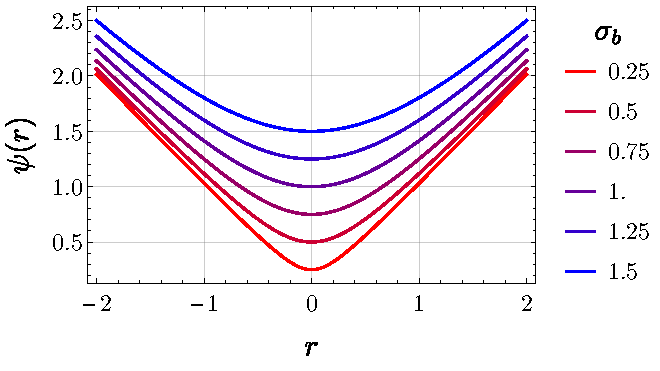
\includegraphics[width=0.58\textwidth]{images/rbf_mq.pdf} \vspace{-1ex} \\ \hline
    \tc{Inverzne multikvadratične \\ (IMQ) \\ \ang{Inverse multiquadrics}
    \\[3ex] $\psi(r) = 1 / \sqrt{r^2+\sigma_b^2}$} & 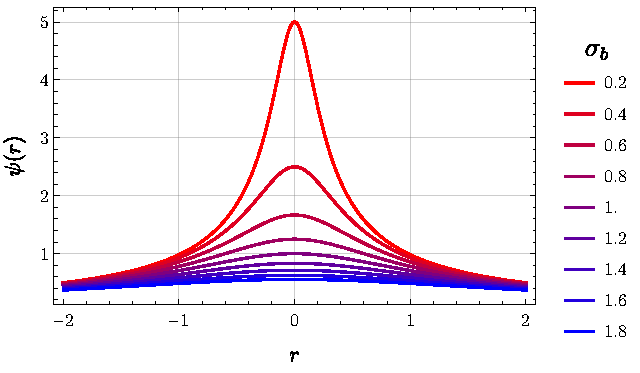
\includegraphics[width=0.58\textwidth]{images/rbf_imq.pdf} \vspace{-1ex} \\ \hline
    \tc{Linearna razdalja (L) \\ \ang{Linear distance} \\[3ex] $\psi(r) = r$} &
    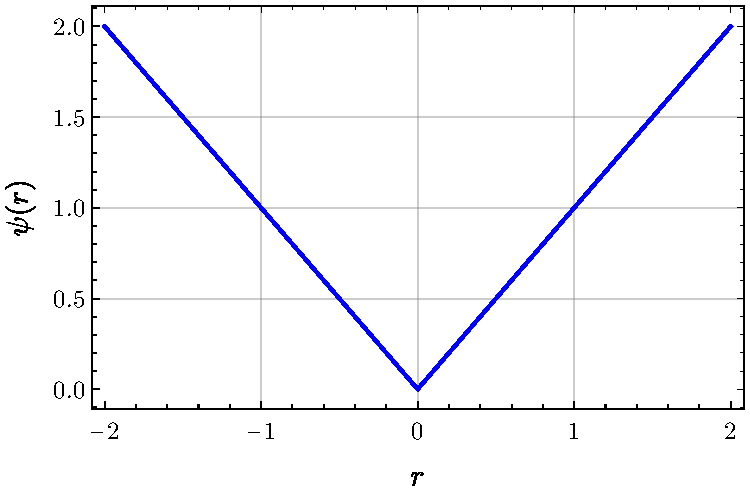
\includegraphics[width=0.49\textwidth]{images/rbf_lin.pdf} \vspace{-1ex} \\ \hline
    \tc{Gaussove funkcije (G) \\ \ang{Gaussians} \\[3ex] $\psi(r) =
    \exp(-(r/\sigma_b)^2)$} & 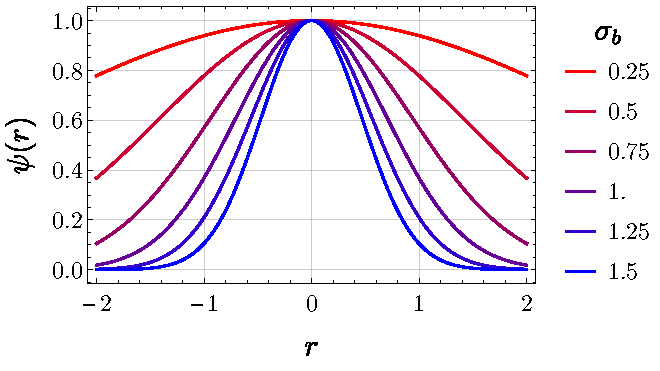
\includegraphics[width=0.58\textwidth]{images/rbf_gau.pdf} \\ \hline
  \end{tabular}
  \caption{Najpogosteje uporabljene radialne bazne funkcije s parametrom oblike
  $\sigma_b$.}
  \label{tab:rbf}
\end{table}

Ko si izberemo neko bazno funkcijo $\psi$, potem za bazne funkcije okoli točke
$p$ vzamemo
\[
  \b b = \{\psi_s; s \in N(p) \}.
\]
Pri izbiri parametra oblike $\sigma_b$ moramo tudi biti do neke mere pazljivi. Izbrati
ga moramo dovolj velikega, da se funkcije ``prekrivajo'', torej tako, da nima
funkcija vrednosti blizu nič pri vseh sosedih razen pri sebi. Hkrati mora biti
parameter dovolj majhen, da sistem~\eqref{eq:shape-system} ni preveč nestabilen.

Pogosto se k bazi radialnih baznih funkcij doda še monome nizkih stopenj, za
boljšo aproksimacijo funkcij, ki so blizu konstantam. Več o kvaliteti,
stabilnosti in redu konvergence aproksimacije z radialnimi baznimi funkcijami
si lahko bralec prebere v~\cite{buhmann2000radial}.

\section{Implementacija}
\label{sec:implementacija}
blah blah~\cite{stroustrup1995c++}.

\section{Osnovni numerični zgledi}
\label{sec:osnovni-zgledi}
V tem razdelku bomo pogledali obnašanje metode na osnovnih numeričnih zgledih,
da si zgradimo intuicijo o njenem delovanju. V nadaljnjem besedilu in na vseh grafih bo
metoda, opisana v razdelku~\ref{sec:numericna-metoda} označena s kratico MLSM
\ang{Meshless Least Squares Method}.
Če ni drugače navedeno, so vse časovne meritve narejene na
prenosnem računalniku s procesorjem
\verb|Intel(R) Core(TM) i7-4700MQ CPU @2.40GHz|
in \unit[16]{GB} DDR3 pomnilnika. Vsi programi so bili prevedeni s
prevajalnikom \verb|g++| verzije 7.1.7 in stikali
\verb|-std=c++14 -O3 -DNDEBUG| na operacijskem sistemu Linux.
Pri paralelizaciji je bila uporabljena knjižnica OpenMP~\cite{dagum1998openmp}
za paralelizacijo z deljenim pomnilnikom.

\subsection{Enodimenzionalni robni problem}
Oglejmo si najprej preprost primer enodimenzionalne Possonove enačbe,
ki smo ga uporabili že za motivacijo izpeljave numerične metode.
Rešujmo problem
\begin{align*}
  u''(x) &= \sin(x), \quad x \in (0, 1) \\
  u(0) &= 0, \\
  u'(1) &= 0,
\end{align*}
ki ima analitično rešitev $u(x) = \cos(1) x - \sin(x)$.
Na sliki~\ref{fig:mlsm-fdm-err} je prikazana konvergenca metode končnih diferenc
in MLSM. Metoda MLSM je bila uporabljena s parametri, pri katerih velja
trditev~\ref{trd:eq-to-fdm}, torej $n=m=3$, $w=1$, $\b b = \{1, x, x^2\}$.
V obeh primerih smo uporabili direktno metodo SuperLU za reševanje sistema
enačb.

\begin{figure}[h]
  \centering
  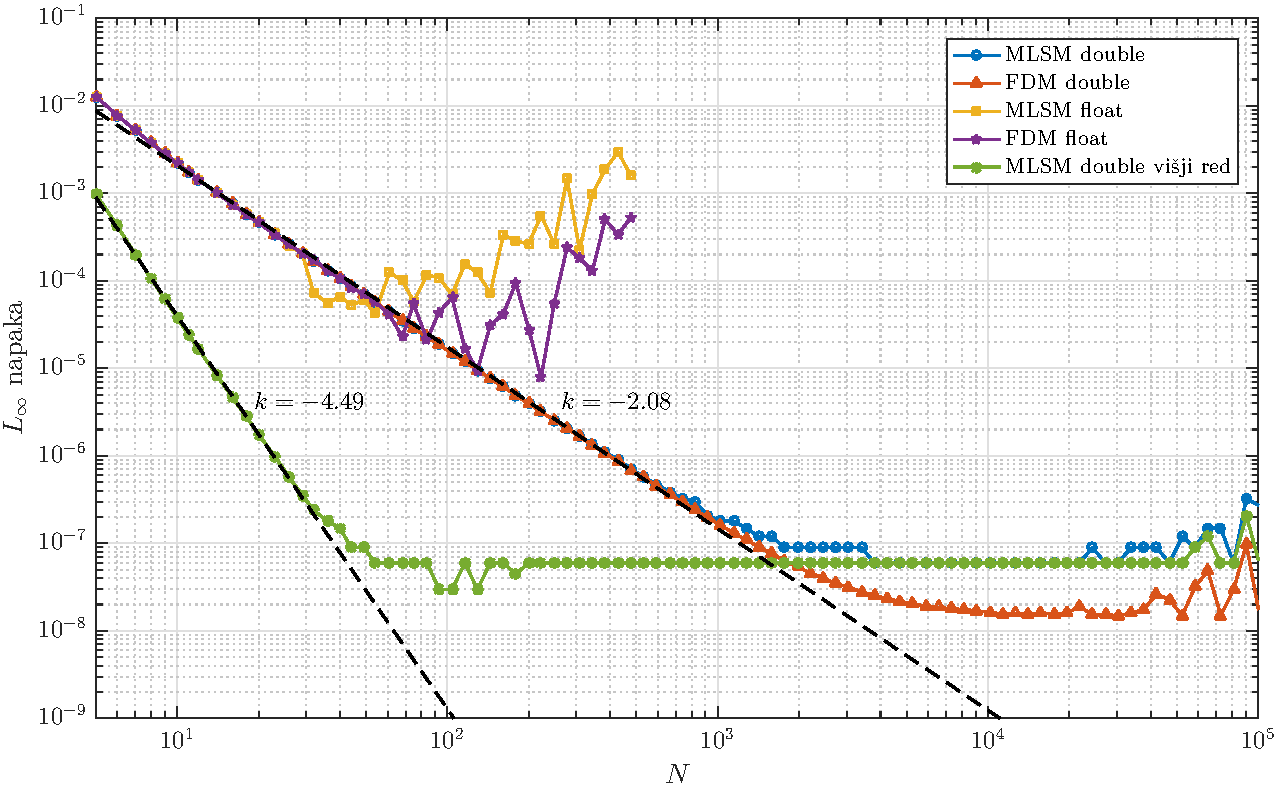
\includegraphics[width=0.8\textwidth]{images/lap1d_convergence.pdf}
  \caption{Napaka FDM in MLSM metode v primerjavi s pravilno rešitvijo.}
  \label{fig:mlsm-fdm-err}
\end{figure}

Na grafu vidimo, da metodi tudi v praksi sovpadata do približno $N=1000$, nato
pa natančnost MLSM postane konstantna, dokler ne pridemo v območje numerične
nestabilnosti. Metoda končnih diferenc pride v območje, ko ne konvergira več z
redom 2 ob približno enaken $N$ kot MLSM, nestabilnosti pa se začnejo kasneje,
med $N = 10^4$ in $N = 10^5$. Hitrejšo nestabilnost MLSM lahko pripišemo
numeričnim napakam pri računanju aproksimacije drugih odvodov, pri FDM namreč v
matriko direktno zapišemo koeficient $-\frac{2}{h^2}$, pri MLSM pa se ta
numerično izračuna.  Iz naklona premice vidimo, da sta obe metodi tudi v praksi
reda~2.

Časovna primerjava obeh metod je prikazana na sliki~\ref{fig:mlsm-fdm-time}.
MLSM je približno konstantno 6-krat počasnejši kot FDM, kot prikazano z
razmerjem, merjenim na desni osi. To je tudi pričakovano, saj MLSM išče
sosede in računa aproksimacije, medtem je to pri FDM vgrajeno v metodo.
Če pri MLSM posebej merimo samo čas, ki ga
porabimo za sestavljanje matrike in reševanje sistema, vidimo, da se skoraj
ujema z časom, porabljenim pri FDM. Minimalno razliko gre pripisati razliki pri
načinu grajenja matrike, saj pri FDM natanko vemo pozicije in število neničelnih
elementov vnaprej, pri MLSM pa v splošnem ne.

\begin{figure}[h]
  \centering
  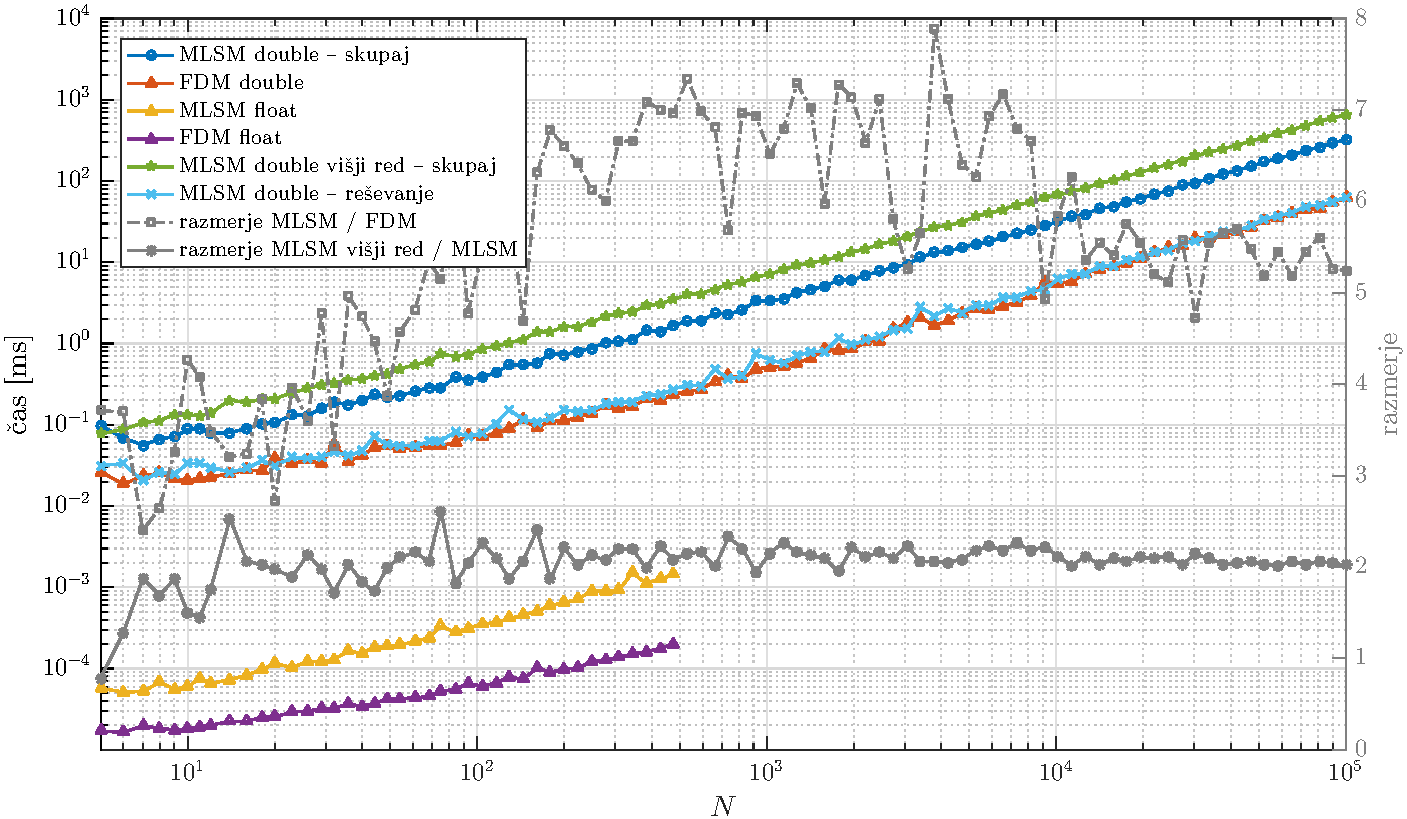
\includegraphics[width=0.8\textwidth]{images/lap1d_times.pdf}
  \caption{Primerjava časa izvajanja MLSM in FDM metod.}
  \label{fig:mlsm-fdm-time}
\end{figure}

\subsection{Poissonova enačba}
Oglejmo si sedaj obnašanje metode na klasični Poissonovi enačbi na kvadratu:
\begin{align}
  \triangle u &= 1, \quad (x, y) \in (0, 1) \times (0, 1)
  \label{eq:poisson-problem} \\
  u(x, 0) &= u(x, 1) = u(0, y) = u(1, y) = 0. \nonumber
\end{align}
Analitično rešitev lahko dobimo s pomočjo separacije spremenljivk in se glasi
\begin{equation}
  u(x, y) =
  -8 \sum_{\substack{k=1 \\ k \text{ lih}}}^\infty \frac{ \sin (k \pi  x) \sinh
  \frac{k \pi  (1-y)}{2} \sinh \frac{k \pi
y}{2}}{\cosh(\frac{k\pi}{2})k^3 \pi ^3}.
  \label{eq:poisson-analytical}
\end{equation}
Za primerjavo z numeričnimi rešitvami bomo uporabili končno vsoto, zato ocenimo
ostanek.
\begin{trditev}
  Za ostanek vrste~\eqref{eq:poisson-analytical} velja
  \[
    \left|-8 \sum_{\substack{k=\ell \\ k \text{ lih}}}^\infty \frac{ \sin (k \pi  x) \sinh
      \frac{k \pi  (1-y)}{2} \sinh \frac{k \pi y}{2}}{\cosh(\frac{k\pi}{2})k^3
      \pi ^3}\right| < -\frac{\psi''(\ell/2)}{4 \pi^3},
  \]
  kjer je $\psi$ digama funkcija.
\end{trditev}
\proof
Ocenjujmo vsak člen vrste posebej. Funkcijo $\sin$ ocenimo z 1, funkcija
$\sinh \frac{k \pi  (1-y)}{2} \sinh \frac{k \pi y}{2}$ ima maksimum na sredini
intervala in jo lahko ocenimo z njeno vrednostjo v $y = \frac{1}{2}$.
Tako nam ostane za oceniti številska vrsta
\[
    -8 \sum_{\substack{k=\ell \\ k \text{ lih}}}^\infty
    \frac{\left(\sinh\frac{k \pi}{4}\right)^2}{\cosh(\frac{k\pi}{2})k^3
    \pi ^3} .
\]
Uporabimo še neenakost $\frac{\left(\sinh\frac{k
\pi}{4}\right)^2}{\cosh(\frac{k\pi}{2})} < \frac{1}{2}$ in dobimo oceno
\[
\left|-8 \sum_{\substack{k=\ell \\ k \text{ lih}}}^\infty \frac{ \sin (k \pi  x) \sinh
      \frac{k \pi  (1-y)}{2} \sinh \frac{k \pi y}{2}}{\cosh(\frac{k\pi}{2})k^3
      \pi ^3}\right| < \frac{4}{\pi^3} \sum_{\substack{k=\ell \\ k \text{ lih}}}^\infty
      \frac{1}{k^3} = -\frac{\psi''(\ell/2)}{4 \pi^3},
\]
kjer je $\psi$ digama funkcija (in posledično $\psi''$ poligama funkcija).
\endproof
Za primer $\ell = 1$  v prejšnji trditvi dobimo oceno
\[
  |u(x, y)| \leq \frac{7 \zeta(3)}{2 \pi^2} \approx 0.1356,
\]
kar drži, v resnici je najbolj ekstremna vrednost $u(1/2, 1/2) \approx -0.7367$.
Kot posledico zgornje trditve lahko izračunamo, da je rep
vrste~\eqref{eq:poisson-analytical} za $\ell = 59$
manjši kot $10^{-5}$, za $\ell = 181$ pa manjši kot $10^{-6}$.
\begin{opomba}
  Računanje izraza \[
    \frac{\sinh \frac{k \pi  (1-y)}{2} \sinh \frac{k \pi
    y}{2}}{\cosh(\frac{k\pi}{2})}
  \] ni numerično stabilno, ko $k$ raste, kajti tako števec kot imenovalec se
  približujeta neskončno, kvocient pa ima končno limito. Ko za želimo izračunati
  numerično je bolje uporabiti stabilnejšo obliko
  \[
    \frac12\left( 1 - \frac{\exp(-k\pi y) + \exp(-k\pi(1-y)) }{1 +
    \exp(-k\pi)}\right),
  \]
  kjer vedno nastopa negativen eksponent.
\end{opomba}

Rešimo problem~\eqref{eq:poisson-problem} numerično, s štirimi različnimi nabori baznih funkcij: monomi,
Gaussovimi funkcijami, multikvadratičnimi in inverznimi multikvadratičnimi.
Za monome vzemimo $n = m = 5$, $m = 6$ in $n=9$ in $m=n=9$, kar sovpada s
primeri iz razdelka~\ref{sec:posebni-primeri}. Za radialne bazne funkcije
vzemimo vedno $n=m$ in sicer vrednosti 5, 9 in 13 za parameter oblike pa
$\sigma_b = 40 r_\chi$. Za utež vzemimo Gaussovo utež z $\sigma_w = r_\chi$.
V vseh primerih je bila za reševanje sistema enačb uporabljena direktna metoda
SuperLU. Iterativni BiCGSTAB algoritem je dal enake rezultate.
Napaka metod je prikazana na sliki~\ref{fig:poisson-square-convergence}.

\begin{figure}[h]
  \centering
  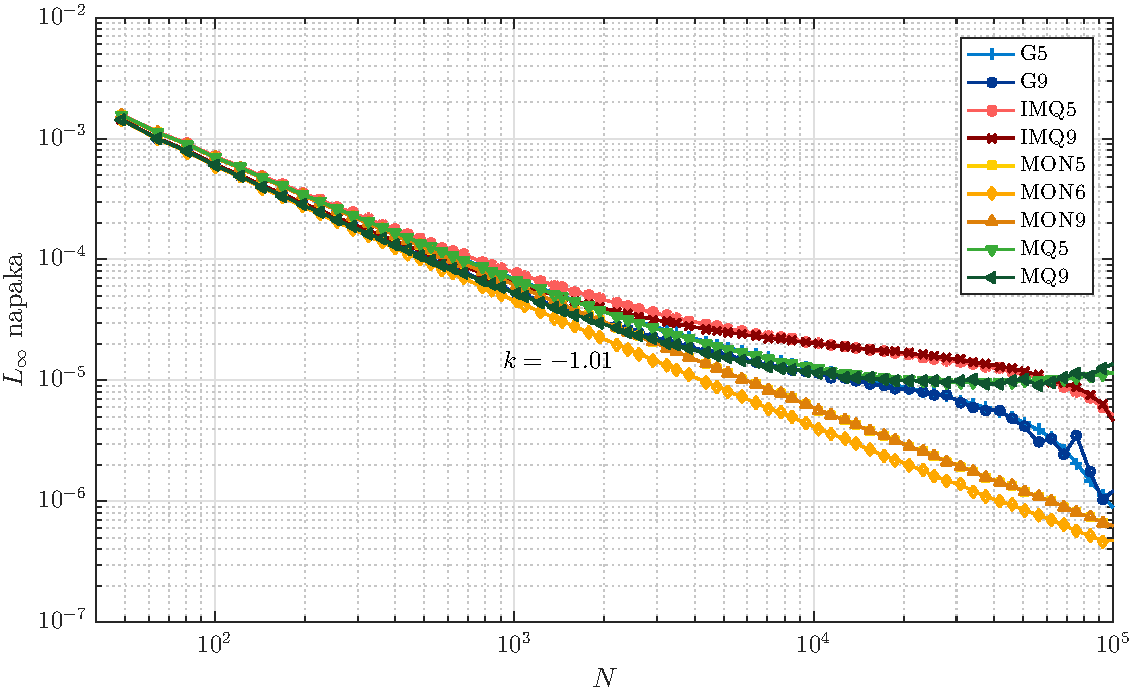
\includegraphics[width=0.8\textwidth]{images/poisson_square_convergence.pdf}
  \caption{Konvergenca MLSM za različne parametre pri reševanju~\eqref{eq:poisson-problem}.}
  \label{fig:poisson-square-convergence}
\end{figure}

\begin{figure}[h]
  \centering
  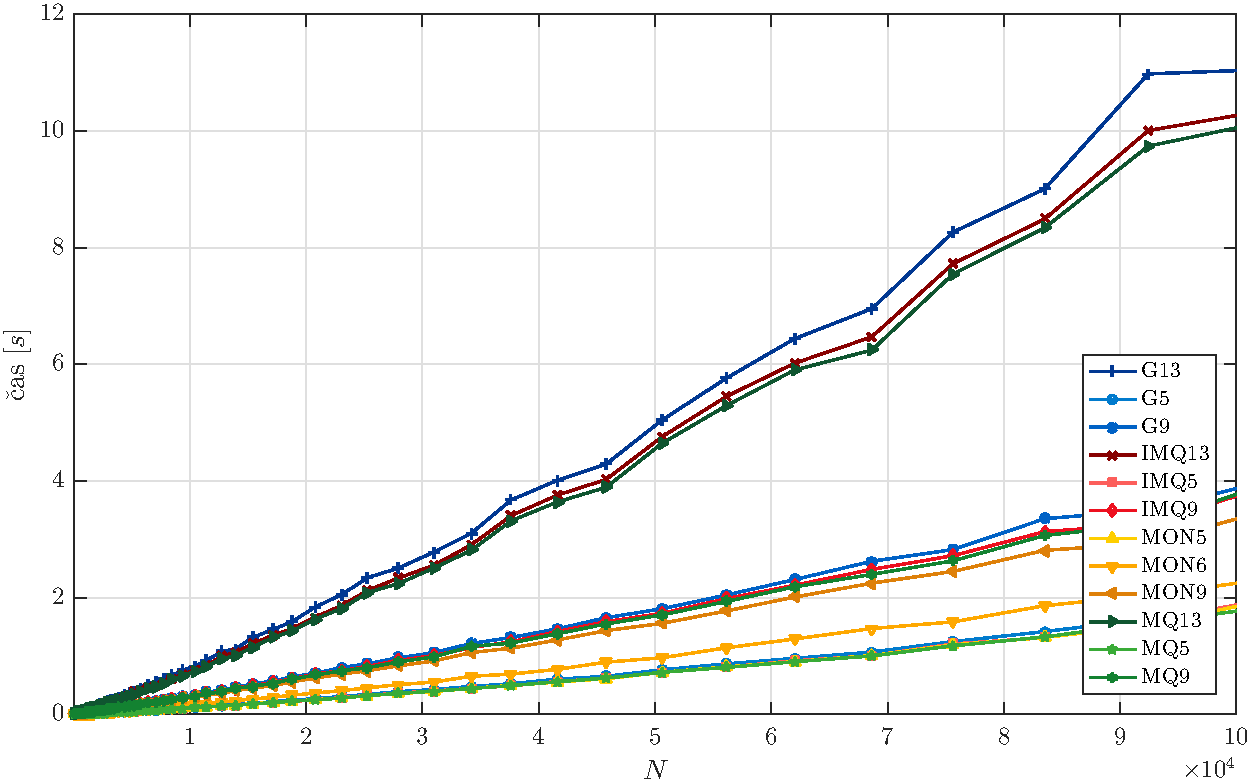
\includegraphics[width=0.8\textwidth]{images/poisson_square_time.pdf}
  \caption{Čas izvajanja za različne izbore parametrov pri reševanju
  problema~\eqref{eq:poisson-problem}.}
  \label{fig:poisson-square-time}
\end{figure}

\begin{figure}[h]
  \centering
  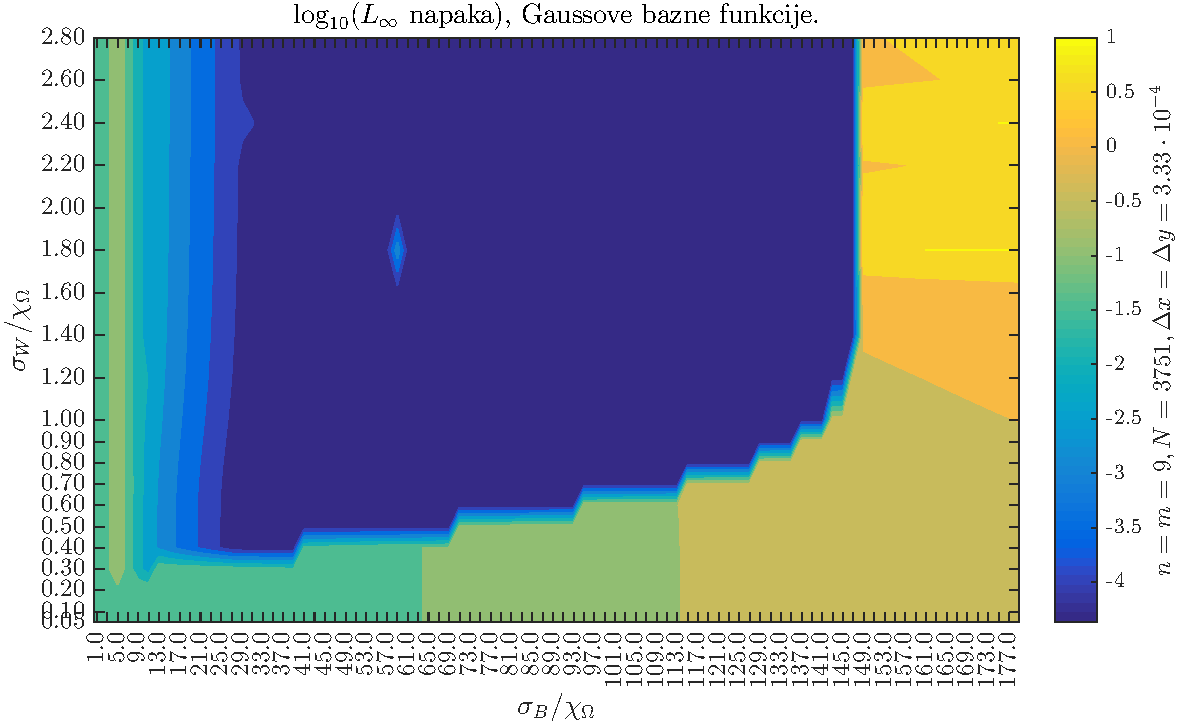
\includegraphics[width=0.8\textwidth]{images/sigma_depedance_error_gau.pdf}
  \caption{Napaka v odvisnosti od $\sigma_b$ in $\sigma_w$ za Gaussove
  funkcije.}
  \label{fig:poisson-square-shapes}
\end{figure}

\begin{figure}[h]
  \centering
  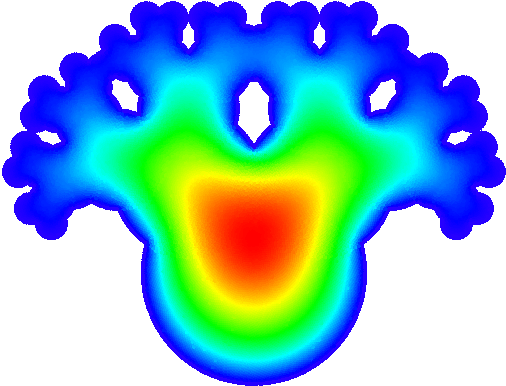
\includegraphics[height=5cm]{images/poisson_weird1.png}
  \hspace{10pt}
  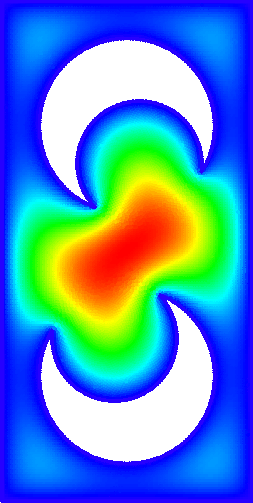
\includegraphics[height=5cm]{images/poisson_weird2.png}
  \hspace{10pt}
  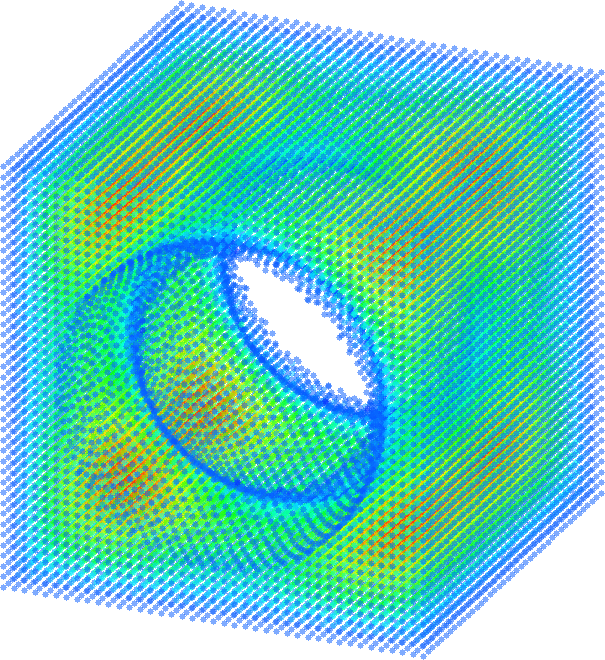
\includegraphics[height=5cm]{images/poisson_weird3.png}
  \caption{Reševanje Poissonove enačbe $\triangle u = 1$ s homogenimi robnimi pogoji na
  zanimivejših domenah.}
  \label{fig:poisson-square-weird}
\end{figure}

\subsection{Hertzov kontaktni problem}
\subsection{FWO case}

\section{Zaključek}

\clearpage
\bibliographystyle{unsrt}
\bibliography{reference}

\end{document}

% vim: set spell spelllang=sl:
